
%%%%%%%%%%%%%%%%%%%%%%%%%%%%%%%%%%%%%%
\documentclass{article}
\usepackage{Sweave}
\usepackage{graphicx}
\usepackage{tabularx}
\usepackage{hyperref}
\usepackage{natbib}
\usepackage{pdflscape}
\usepackage{array}
\usepackage{gensymb}
\usepackage{amsmath}
\usepackage{longtable}
\usepackage{xr}
\usepackage[small]{caption}

\setkeys{Gin}{width=0.8\textwidth}
\setlength{\captionmargin}{30pt}
\setlength{\abovecaptionskip}{10pt}
\setlength{\belowcaptionskip}{10pt}
 \topmargin -1.5cm        
 \oddsidemargin -0.04cm   
 \evensidemargin -0.04cm
 \textwidth 16.59cm
 \textheight 21.94cm 
 \parskip 7.2pt          
 \parindent 0pt
\usepackage{setspace}
\externaldocument{/Users/aileneettinger/Documents/GitHub/ospree/docs/budburst/budburstms}
\externaldocument{/Users/aileneettinger/Documents/GitHub/ospree/docs/budburst/budburst_extdat}
%%%%%%%%%%%%%%%%%%%%%%%%%%%%%%%%%%%%%%

\begin{document}

\bibliographystyle{..//..//refs/bibstyles/naturemag}
\title{Supplemental Materials:  Winter temperatures predominate in spring phenological responses to warming} 

\author{A. K. Ettinger, C. J. Chamberlain, I. Morales-Castilla, D. M. Buonaiuto, D. F. B. Flynn, \\ T. Savas, J. A. Samaha \& E. M. Wolkovich}
\date{} 
\maketitle  
%%%%%%%%%%%%%%%%%%%%%%%%%%%%%%%%%%%%%%%%%%%%%%%%%%%
\renewcommand{\thetable}{S\arabic{table}}
\renewcommand{\thefigure}{S\arabic{figure}}

\section*{Applying our model to Central European data}

Our results integrate over a large range of chilling, forcing, and photoperiod conditions (\emph{e.g.}, forcing treatment temperatures ranged from 0-32\degree C and chilling temperatures ranged from -10-16\degree C in experiments, as defined by each study's authors, Figs. \ref{fig:3dfieldchillutah}, \ref{fig:3dexpchillutah}). We wished to understand how our findings may apply to conditions more commonly found in nature, especially where conditions often vary dramatically from those applied in controlled environment experiments. For example, very low amounts of chilling can be applied in experiments compared to the higher amounts of natural chilling found in many temperate areas (Fig. \ref{fig:chillexpfield}). Additionally, chilling temperature and total chilling are more correlated in nature than in experimental conditions (Fig. \ref{fig:chillexpfield}). Further, given the importance of chilling and forcing combined with the fact that seasons do not always warm uniformly with climate change \emph{\citep{vautard2014,eea2019}}, we also wished to understand how warming in the winter, spring, or both seasons would shift budburst timing. Given these goals we focused on applying our model estimates to defined levels of warming layered onto historical climate. Alternative approaches, such as using climate projections from global circulation models, would have hindered our efforts to understand degrees of warming in different seasons. Further, we emphasize that our predictions are not designed to be accurate forecasts of future budburst dates, even for the locations for which we use historical climate and budburst data. Rather, they are designed to provide insights into how natural conditions can differ from experimental conditions, and to provide guidance on how much varying effects of winter and spring warming together will shape future budburst timing.

\par We applied our model to Central Europe, a well-studied area for phenology, which has both relatively long-term daily temperature data and budburst data. We selected sites that are part of the Pan European Phenology Project (PEP725, \url{http://www.pep725.eu}) and included data for two common European species that are prevalent in the OSPREE database: \emph{Betula pendula} (silver birch) and \emph{Fagus sylvatica} (European beech) \emph{\citep{Templ2018}}. We used a European-wide gridded climate dataset \emph{\citep[{\normalfont E-OBS},][]{cornes2018}} to extract daily minimum and maximum temperature for the grid cells where observations of leafout for these two species were available. We extracted temperature data from 1951 through 1960 (selected as a pre-warming time period) and used these data to estimate annual values for total winter chilling (from 1 September through 30 April, in Utah units, using the R package \texttt{chillR}, see in the \emph{Estimating chilling} section of the \emph{Methods}) and mean spring forcing estimated as the mean temperature from 1 March through 30 April. We inputted these estimates for chilling and forcing into our main model, and set photoperiod to the daylength on the mean day of leafout across the PEP725 observations from 1951 through 1960. This yielded estimates of budburst under ``pre-warming conditions.'' We then investigated model predictions of budburst given different levels of warming (from 1-7\degree C) above this baseline, including a full matrix of altered total chilling and forcing estimates (Figs. \ref{fig:3dfieldchillutah}, \ref{fig:3dexpchillutah}). 
\par We applied our model at all latitudes and longitudes included in the PEP725 database between 1951 and 1960 for \emph{Betula pendula} (Fig. \ref{fig:foremap}). We selected two of these sites for \emph{Betula pendula}, as well as two sites where \emph{Fagus sylvatica} occurs, to compare budburst responses across species that differ in their responses to chilling, forcing, and photoperiod, as well as sites that differ in baseline climate (Figs. \ref{fig:betfag3d}, \ref{fig:foremap}, \ref{fig:betfag2d}, \ref{fig:chillfore}).

\par We also applied our latitude model to Central Europe, focusing on PEP725 sites where \emph{Fagus sylvatica} leafout data were available from 1951-1960. We fit the model to three sites that differed in latitude, following the approach above for estimating baseline chilling and forcing for these sites (Fig. \ref{fig:fagsyllat}) and applying warming levels ranging from 1 to 7\degree C.   For each site, we used as a baseline photoperiod the daylength on the mean day of leafout from PEP725 observations between 1951 and 1960. We then further estimated potential changes in photoperiod due to advancing phenology. To do this, we first estimated the shift in days to budburst, as described above.
We then used this budburst date to estimate the change in photoperiod between the day of year during the pre- and post-warming periods and then re-fit the model with this new photoperiod (Fig. \ref{fig:fagsyllat}). 

\par Note that, as described in the \emph{Models} section of the \emph{Methods}, our days to budburst estimate is the days to budburst since forcing conditions were applied in the experiment, which we stress is not necessarily the days to budburst after the start of ecodormancy \emph{\citep{chuine2016}}.

\section*{Potential statistical artifacts in declines of temperature sensitivity in observational long-term data} 

Since our model results do not predict a dramatic decline in temperature sensitivity in Central Europe, as has been observed \emph{\citep[e.g.,][]{fu2015}}, we tested whether observed declines could instead be due to a statistical artifact. Researchers today commonly estimate temperature sensitivity via a linear regression of annual budburst date versus mean or other aggregated metrics of spring temperature yielding estimates in days/$^{\circ}$C. However, if warming produces systematically higher daily temperatures this method will inherently estimate lower sensitivities, because the ``days'' unit will effectively have increased in the thermal sum it represents (that is, the unit of ``days'' is non-stationary in recent decades).
\par To test this hypothesis we compared observed trends with simple simulations. First, we collated PEP725 data \emph{\citep{Templ2018}} for \emph{Betula pendula} for all sites with leafout data each year from two 10-year time-periods: a period before significant anthropogenic warming (1951-1960) and a period with significant warming \emph{\citep[{\normalfont 2001-2010, see}][]{IPCC:2014sm}}. We used leafout data (BBCH=11; which is defined as ``leaf unfolding (first visible leaf stalk)'' in the PEP725 database) instead of budburst (BBCH=7; defined as ``Beginning of sprouting'') as leafout data are far more common in the PEP725 database. Next, we simulated budburst data with constant cues. For this, we did not include any chilling or photoperiod cues, but assumed budburst occurred after a certain thermal sum, estimated via growing degree days with a base temperature of 0$^{\circ}$C. We then estimated temperature sensitivity (days/$^{\circ}$C) and the difference in these estimates given different levels of spring warming. For the simulations shown here we used a GDD (growing degree day) requirement of 150, a base mean spring temperature of 6$^{\circ}$C with a variance of 3$^{\circ}$C, and estimated temperature sensitivity for 10-year periods for 45 simulated sites (these values were chosen to best match the PEP725 data, but note that the general findings are robust to other combinations of these parameter values).

\par As expected, temperature sensitivity estimates for \emph{Betula pendula} from PEP725 declined across the two time periods in step with warming. Across the sites studied here, we estimated a decline of 0.8$\pm$0.3 days/$^{\circ}$C (comparing 2001-2010 and 1951-1960) and 1.1$\pm$0.2$^{\circ}$C warming; this estimate was very similar to simulations given constant cues and 1$^{\circ}$C warming (Fig. \ref{fig:pepsims}). 

\par Additionally, several other metrics suggest declines may be more statistical than biological. Research suggests substantial declines in chilling---that could lead to observed shifts in sensitivity to warming---should increase variance in leafout timing \emph{\citep{ford2016}}. In contrast, in both the real and simulated data, variance in leafout date declined over time---this would be expected if plants use a thermal sum threshold of forcing to leaf out and warming produces systematically warmer days. In the PEP725 data we found a decline in leafout variance of 58\% (in recent years compared to earlier years), compared to a decline of 37\% in the simulations. Additionally we found little change in accumulated chilling (1 September - 1 March of each year) in the PEP725 data across the two time points (2247$\pm$31 Utah units in 1951-1960, compared to 2236$\pm$20 Utah units in 2001-2010), further suggesting that shifts in chilling do not explain the declining sensitivities. Simple plots of the chilling and forcing required for budburst suggest very low chilling is often required to dramatically increase the forcing required for budburst (Figs. \ref{fig:pep}, \ref{fig:pepgddchill}). 
\par We also tested whether the observed declines in sensitivity could be explained via the absolute sliding time window (SWA) approach \emph{\citep{simmonds2019}}. Sliding window analyses determine the optimum time period in which environmental factors---in this case, temperature---influence a phenological response, such as leafout. Various iterations of linear models are run to test different durations and calendar positions for the time window to be open and the best model is then selected based on explanatory power \emph{\citep{simmonds2019, Bailey2016}}.  We again used collated data from the PEP725 data \emph{\citep{Templ2018}} for \emph{Betula pendula} for all sites with leafout data for each year within the same time periods as above: 1951-1960 (pre-warming) and 2001-2010 (post-warming). We then extracted daily minimum and daily maximum climate data from E-OBS \emph{\citep{cornes2018}} for each site. Using the R package \texttt{climwin} \emph{\citep{Bailey2016,vandepol2016}} and following code from \emph{\citep{simmonds2019}}, we tested the temperature sensitivity of leaf-out during the two time periods.  
\par We found that the SWA approach yielded consistent results with our previous analyses: higher sensitivity during the pre-warming time period (Table \ref{tab:clim}), though when adjusted for the increasing thermal sum per day with warming there was little difference in sensitivity to forcing across the two time-periods (Table \ref{tab:swa}). In addition, during the post-warming time period, the window was open for 18 fewer days and exhibited lower variance than in the pre-warming time period (Table \ref{tab:swa}). 

\par This potential artifact adds to existing research that has documented the statistical challenges of accurately estimating temperature sensitivities from long-term data \emph{\citep{gusewell2017,clark2014a}} and may be overcome by some methods. Research that measures sensitivity as a thermal sum or other temperature metric (\emph{e.g.}, GDD) until leafout should be less vulnerable to this artifact. Indeed, in the PEP725 data we found little difference across the two time-periods in GDD (68.7$\pm$2.6 in 1950-1960 versus 61.5$\pm$2.0 in 2000-2010 for GDD calculated from January 1st to leafout with a base temperature of 0$^{\circ}$C; and a mean temperature in the 30 days before leafout of 6.8$^{\circ}$C$\pm$0.1 in 1950-1960 versus 6.6$^{\circ}$C$\pm$0.1). Methods such as these (that accumulate thermal temperatures until event date) are vulnerable to other issues: as researchers must select the day to start accumulating or averaging temperatures, these methods should work best when the start date is always after endodormancy break, when plants are most responsive to forcing \emph{\citep{chuine2016}}. As climate change may push endodormancy break later and later in some regions, this method could inaccurately attribute changes in other cues to shifts in forcing \emph{\citep{gusewell2017}}. Without measures of endodormancy break \emph{\citep{chuine2016}}, we suggest efforts to accurately estimate cues from long-term observational data may be difficult or impossible without additional physiological information from controlled environment experiments.


%\bibliography{..//..//refs/ospreebibplus.bib}

\newpage
\begin{thebibliography}{10}
\expandafter\ifx\csname url\endcsname\relax
  \def\url#1{\texttt{#1}}\fi
\expandafter\ifx\csname urlprefix\endcsname\relax\def\urlprefix{URL }\fi
\providecommand{\bibinfo}[2]{#2}
\providecommand{\eprint}[2][]{\url{#2}}

\bibitem{vautard2014}
\bibinfo{author}{Vautard, R.} \emph{et~al.}
\newblock \bibinfo{title}{{The European climate under a 2 \degree C global
  warming}}.
\newblock \emph{\bibinfo{journal}{Environmental Research Letters}}
  \textbf{\bibinfo{volume}{9}}, \bibinfo{pages}{034006} (\bibinfo{year}{2014}).

\bibitem{eea2019}
\bibinfo{author}{Agency, D.} \& \bibinfo{author}{K{\"o}rner, C.}
\newblock \bibinfo{title}{Global and {E}uropean temperature}
  (\bibinfo{year}{2019}).

\bibitem{Templ2018}
\bibinfo{author}{Templ, B.} \emph{et~al.}
\newblock \bibinfo{title}{{Pan European Phenological database (PEP725): a
  single point of access for European data}}.
\newblock \emph{\bibinfo{journal}{International Journal of Biometeorology}}
  \textbf{\bibinfo{volume}{62}}, \bibinfo{pages}{1109--1113}
  (\bibinfo{year}{2018}).

\bibitem{cornes2018}
\bibinfo{author}{Cornes, R.~C.}, \bibinfo{author}{van~der Schrier, G.},
  \bibinfo{author}{van~den Besselaar, E.~J.} \& \bibinfo{author}{Jones, P.~D.}
\newblock \bibinfo{title}{An ensemble version of the {E-OBS} temperature and
  precipitation data sets}.
\newblock \emph{\bibinfo{journal}{Journal of Geophysical Research:
  Atmospheres}} \textbf{\bibinfo{volume}{123}}, \bibinfo{pages}{9391--9409}
  (\bibinfo{year}{2018}).

\bibitem{chuine2016}
\bibinfo{author}{Chuine, I.} \emph{et~al.}
\newblock \bibinfo{title}{Can phenological models predict tree phenology
  accurately in the future? {T}he unrevealed hurdle of endodormancy break}.
\newblock \emph{\bibinfo{journal}{Global Change Biology}}
  \textbf{\bibinfo{volume}{22}}, \bibinfo{pages}{3444--3460}
  (\bibinfo{year}{2016}).

\bibitem{fu2015}
\bibinfo{author}{Fu, Y. S.~H.} \emph{et~al.}
\newblock \bibinfo{title}{Declining global warming effects on the phenology of
  spring leaf unfolding}.
\newblock \emph{\bibinfo{journal}{Nature}} \textbf{\bibinfo{volume}{526}},
  \bibinfo{pages}{104--107} (\bibinfo{year}{2015}).

\bibitem{IPCC:2014sm}
\bibinfo{author}{IPCC}.
\newblock \emph{\bibinfo{title}{Climate Change 2014: Impacts, Adaptation, and
  Vulnerability}} (\bibinfo{publisher}{Cambridge University Press},
  \bibinfo{address}{Cambridge, United Kingdom and New York, NY, USA},
  \bibinfo{year}{2014}).

\bibitem{ford2016}
\bibinfo{author}{Ford, K.~R.}, \bibinfo{author}{Harrington, C.~A.},
  \bibinfo{author}{Bansal, S.}, \bibinfo{author}{Gould, J., Peter} \&
  \bibinfo{author}{St.~Clair, J.~B.}
\newblock \bibinfo{title}{Will changes in phenology track climate change? {A}
  study of growth initiation timing in coast {Douglas--fir}}.
\newblock \emph{\bibinfo{journal}{Global Change Biology}}
  \textbf{\bibinfo{volume}{22}}, \bibinfo{pages}{3712--3723}
  (\bibinfo{year}{2016}).

\bibitem{simmonds2019}
\bibinfo{author}{Simmonds, E.~G.}, \bibinfo{author}{Cole, E.~F.} \&
  \bibinfo{author}{Sheldon, B.~C.}
\newblock \bibinfo{title}{Cue identification in phenology: a case study of the
  predictive performance of current statistical tools}.
\newblock \emph{\bibinfo{journal}{Journal of Animal Ecology}}
  (\bibinfo{year}{2019}).

\bibitem{Bailey2016}
\bibinfo{author}{Bailey, L.~D.} \& \bibinfo{author}{van~de Pol, M.}
\newblock \bibinfo{title}{climwin: An r toolbox for climate window analysis}.
\newblock \emph{\bibinfo{journal}{PLOS ONE}} \textbf{\bibinfo{volume}{11}},
  \bibinfo{pages}{1--27} (\bibinfo{year}{2016}).

\bibitem{vandepol2016}
\bibinfo{author}{van~de Pol, M.} \emph{et~al.}
\newblock \bibinfo{title}{Identifying the best climatic predictors in ecology
  and evolution}.
\newblock \emph{\bibinfo{journal}{Methods in Ecology and Evolution}}
  \textbf{\bibinfo{volume}{7}}, \bibinfo{pages}{1246--1257}
  (\bibinfo{year}{2016}).
\newblock
  \eprint{https://besjournals.onlinelibrary.wiley.com/doi/pdf/10.1111/2041-210X.12590}.

\bibitem{gusewell2017}
\bibinfo{author}{G{\"u}sewell, S.}, \bibinfo{author}{Furrer, R.},
  \bibinfo{author}{Gehrig, R.} \& \bibinfo{author}{Pietragalla, B.}
\newblock \bibinfo{title}{{Changes in temperature sensitivity of spring
  phenology with recent climate warming in Switzerland are related to shifts of
  the preseason}}.
\newblock \emph{\bibinfo{journal}{Global Change Biology}}
  \textbf{\bibinfo{volume}{23}}, \bibinfo{pages}{5189--5202}
  (\bibinfo{year}{2017}).

\bibitem{clark2014a}
\bibinfo{author}{Clark, J.~S.}, \bibinfo{author}{Melillo, J.},
  \bibinfo{author}{Mohan, J.} \& \bibinfo{author}{Salk, C.}
\newblock \bibinfo{title}{The seasonal timing of warming that controls onset of
  the growing season}.
\newblock \emph{\bibinfo{journal}{Global Change Biology}}
  \textbf{\bibinfo{volume}{20}}, \bibinfo{pages}{1136--1145}
  (\bibinfo{year}{2014}).

\bibitem{Basler:2012}
\bibinfo{author}{Basler, D.} \& \bibinfo{author}{K{\"o}rner, C.}
\newblock \bibinfo{title}{Photoperiod sensitivity of bud burst in 14 temperate
  forest tree species}.
\newblock \emph{\bibinfo{journal}{Agricultural and Forest Meteorology}}
  \textbf{\bibinfo{volume}{165}}, \bibinfo{pages}{73--81}
  (\bibinfo{year}{2012}).

\bibitem{Basler:2014aa}
\bibinfo{author}{Basler, D.} \& \bibinfo{author}{K{\"o}rner, C.}
\newblock \bibinfo{title}{Photoperiod and temperature responses of bud swelling
  and bud burst in four temperate forest tree species}.
\newblock \emph{\bibinfo{journal}{Tree Physiology}}
  \textbf{\bibinfo{volume}{34}}, \bibinfo{pages}{377--388}
  (\bibinfo{year}{2014}).

\bibitem{Biasi:2012}
\bibinfo{author}{Biasi, L.}, \bibinfo{author}{Zanette, F.} \&
  \bibinfo{author}{Carvalho, R.}
\newblock \bibinfo{title}{Dormancy dynamics of grape and kiwifruit buds in a
  region of low chill occurrence}.
\newblock In \emph{\bibinfo{booktitle}{XXVIII International Horticultural
  Congress on Science and Horticulture for People (IHC2010): International
  Symposium on Plant 932}}, \bibinfo{pages}{507--512} (\bibinfo{year}{2012}).

\bibitem{Caffarra:2011a}
\bibinfo{author}{Caffarra, A.} \& \bibinfo{author}{Donnelly, A.}
\newblock \bibinfo{title}{The ecological significance of phenology in four
  different tree species: effects of light and temperature on bud burst}.
\newblock \emph{\bibinfo{journal}{International Journal of Biometeorology}}
  \textbf{\bibinfo{volume}{55}}, \bibinfo{pages}{711--721}
  (\bibinfo{year}{2011}).

\bibitem{Caffarra:2011b}
\bibinfo{author}{Caffarra, A.}, \bibinfo{author}{Donnelly, A.},
  \bibinfo{author}{Chuine, I.} \& \bibinfo{author}{Jones, M.~B.}
\newblock \bibinfo{title}{{Modelling the timing of \textit{Betula pubescens}
  bud-burst. I. Temperature and photoperiod: A conceptual model}}.
\newblock \emph{\bibinfo{journal}{Climate Research}}
  \textbf{\bibinfo{volume}{46}}, \bibinfo{pages}{147} (\bibinfo{year}{2011}).

\bibitem{Calme:1994aa}
\bibinfo{author}{Calm{\'e}, S.}, \bibinfo{author}{Bigras, F.~J.},
  \bibinfo{author}{Margolis, H.~A.} \& \bibinfo{author}{H{\'e}bert, C.}
\newblock \bibinfo{title}{Frost tolerance and bud dormancy of container-grown
  yellow birch, red oak and sugar maple seedlings}.
\newblock \emph{\bibinfo{journal}{Tree Physiology}}
  \textbf{\bibinfo{volume}{14}}, \bibinfo{pages}{1313--1325}
  (\bibinfo{year}{1994}).

\bibitem{Campbell:1975aa}
\bibinfo{author}{Campbell, R.~K.} \& \bibinfo{author}{Sugano, A.~I.}
\newblock \bibinfo{title}{{Phenology of bud burst in Douglas-fir related to
  provenance, photoperiod, chilling, and flushing temperature}}.
\newblock \emph{\bibinfo{journal}{Botanical Gazette}} \bibinfo{pages}{290--298}
  (\bibinfo{year}{1975}).

\bibitem{Chavarria:2009aa}
\bibinfo{author}{Chavarria, G.} \emph{et~al.}
\newblock \bibinfo{title}{Mild temperatures on bud breaking dormancy in
  peaches}.
\newblock \emph{\bibinfo{journal}{Ci{\^e}ncia Rural}}
  \textbf{\bibinfo{volume}{39}}, \bibinfo{pages}{2016--2021}
  (\bibinfo{year}{2009}).

\bibitem{Cook:2000aa}
\bibinfo{author}{Cook, C.} \& \bibinfo{author}{Jacobs, G.}
\newblock \bibinfo{title}{Progression of apple (malus$\times$ domestica borkh.)
  bud dormancy in two mild winter climates}.
\newblock \emph{\bibinfo{journal}{The Journal of Horticultural Science and
  Biotechnology}} \textbf{\bibinfo{volume}{75}}, \bibinfo{pages}{233--236}
  (\bibinfo{year}{2000}).

\bibitem{Falusi:2003aa}
\bibinfo{author}{Falusi, M.} \& \bibinfo{author}{Calamassi, R.}
\newblock \bibinfo{title}{{Dormancy of \emph{Fagus sylvatica} L. buds III.
  Temperature and hormones in the evolution of dormancy in one-node cuttings}}.
\newblock \emph{\bibinfo{journal}{Plant Biosystems-An International Journal
  Dealing with all Aspects of Plant Biology}} \textbf{\bibinfo{volume}{137}},
  \bibinfo{pages}{185--191} (\bibinfo{year}{2003}).

\bibitem{Falusi:1990aa}
\bibinfo{author}{Falusi, M.} \& \bibinfo{author}{Calamassi, R.}
\newblock \bibinfo{title}{{Bud dormancy in beech (\textit{Fagus sylvatica} L.).
  Effect of chilling and photoperiod on dormancy release of beech seedlings}}.
\newblock \emph{\bibinfo{journal}{Tree Physiology}}
  \textbf{\bibinfo{volume}{6}}, \bibinfo{pages}{429--438}
  (\bibinfo{year}{1990}).

\bibitem{Falusi:1996aa}
\bibinfo{author}{Falusi, M.} \& \bibinfo{author}{Calamassi, R.}
\newblock \bibinfo{title}{{Geographic variation and bud dormancy in beech
  seedlings (\emph{Fagus sylvatica} L)}}.
\newblock In \emph{\bibinfo{booktitle}{Annales des Sciences foresti{\`e}res}},
  vol.~\bibinfo{volume}{53}, \bibinfo{pages}{967--979} (\bibinfo{publisher}{EDP
  Sciences}, \bibinfo{year}{1996}).

\bibitem{Falusi:1997aa}
\bibinfo{author}{Falusi, M.} \& \bibinfo{author}{Calamassi, R.}
\newblock \bibinfo{title}{{Bud dormancy in \emph{Fagus sylvatica} L. II. The
  evolution of dormancy in seedlings and one-node cuttings}}.
\newblock \emph{\bibinfo{journal}{Plant Biosystems-An International Journal
  Dealing with all Aspects of Plant Biology}} \textbf{\bibinfo{volume}{131}},
  \bibinfo{pages}{143--148} (\bibinfo{year}{1997}).

\bibitem{Ghelardini:2010aa}
\bibinfo{author}{Ghelardini, L.}, \bibinfo{author}{Santini, A.},
  \bibinfo{author}{Black-Samuelsson, S.}, \bibinfo{author}{Myking, T.} \&
  \bibinfo{author}{Falusi, M.}
\newblock \bibinfo{title}{Bud dormancy release in elm ( {\emph{ulmus}} spp.)
  clones---a case study of photoperiod and temperature responses}.
\newblock \emph{\bibinfo{journal}{Tree physiology}}
  \textbf{\bibinfo{volume}{30}}, \bibinfo{pages}{264--274}
  (\bibinfo{year}{2010}).

\bibitem{Gianfagna:1985aa}
\bibinfo{author}{Gianfagna, T.} \& \bibinfo{author}{Mehlenbacher, S.}
\newblock \bibinfo{title}{Importance of heat requirement for bud break and time
  of flowering in apple}.
\newblock \emph{\bibinfo{journal}{HortScience}} \textbf{\bibinfo{volume}{20}},
  \bibinfo{pages}{909--911} (\bibinfo{year}{1985}).

\bibitem{Gomory:2015aa}
\bibinfo{author}{G{\"o}m{\"o}ry, D.}, \bibinfo{author}{Foffov{\'a}, E.},
  \bibinfo{author}{Longauer, R.} \& \bibinfo{author}{Krajmerov{\'a}, D.}
\newblock \bibinfo{title}{{Memory effects associated with early-growth
  environment in Norway spruce and European larch}}.
\newblock \emph{\bibinfo{journal}{European Journal of Forest Research}}
  \textbf{\bibinfo{volume}{134}}, \bibinfo{pages}{89--97}
  (\bibinfo{year}{2015}).

\bibitem{Guak:1998aa}
\bibinfo{author}{Guak, S.}, \bibinfo{author}{Olsyzk, D.~M.},
  \bibinfo{author}{Fuchigami, L.~H.} \& \bibinfo{author}{Tingey, D.~T.}
\newblock \bibinfo{title}{Effects of elevated {CO}2 and temperature on cold
  hardiness and spring bud burst and growth in douglas-fir (\emph{Pseudotsuga
  menziesii})}.
\newblock \emph{\bibinfo{journal}{Tree Physiology}}
  \textbf{\bibinfo{volume}{18}}, \bibinfo{pages}{671--679}
  (\bibinfo{year}{1998}).

\bibitem{guerriero:1990}
\bibinfo{author}{Guerriero, P.}, \bibinfo{author}{Scalabrelli, G.} \&
  \bibinfo{author}{Grazzini, G.}
\newblock \bibinfo{title}{Chilling effect on inhibition removal in kiwifruit
  dormant lateral buds}.
\newblock In \emph{\bibinfo{booktitle}{I International Symposium on Kiwifruit
  282}}, \bibinfo{pages}{79--86} (\bibinfo{year}{1990}).

\bibitem{Heide:2012aa}
\bibinfo{author}{Heide, O.~M.} \& \bibinfo{author}{S{\o}nsteby, A.}
\newblock \bibinfo{title}{{Floral initiation in black currant cultivars
  (\emph{Ribes nigrum} L.): Effects of plant size, photoperiod, temperature,
  and duration of short day exposure}}.
\newblock \emph{\bibinfo{journal}{Scientia Horticulturae}}
  \textbf{\bibinfo{volume}{138}}, \bibinfo{pages}{64--72}
  (\bibinfo{year}{2012}).

\bibitem{Heide:1993}
\bibinfo{author}{Heide, O.}
\newblock \bibinfo{title}{Daylength and thermal time responses of budburst
  during dormancy release in some northern deciduous trees}.
\newblock \emph{\bibinfo{journal}{Physiologia Plantarum}}
  \textbf{\bibinfo{volume}{88}}, \bibinfo{pages}{531--540}
  (\bibinfo{year}{1993}).

\bibitem{Heide:1993a}
\bibinfo{author}{Heide, O.}
\newblock \bibinfo{title}{{Dormancy release in beech buds (\textit{Fagus
  sylvatica}) requires both chilling and long days}}.
\newblock \emph{\bibinfo{journal}{Physiologia Plantarum}}
  \textbf{\bibinfo{volume}{89}}, \bibinfo{pages}{187--191}
  (\bibinfo{year}{1993}).

\bibitem{Jones:2012}
\bibinfo{author}{Jones, H.}, \bibinfo{author}{Hillis, R.},
  \bibinfo{author}{Gordon, S.} \& \bibinfo{author}{Brennan, R.}
\newblock \bibinfo{title}{{An approach to the determination of winter chill
  requirements for different \emph{Ribes} cultivars}}.
\newblock \emph{\bibinfo{journal}{Plant Biology}}
  \textbf{\bibinfo{volume}{15}}, \bibinfo{pages}{18--27}
  (\bibinfo{year}{2012}).

\bibitem{Laube:2014a}
\bibinfo{author}{Laube, J.} \emph{et~al.}
\newblock \bibinfo{title}{Chilling outweighs photoperiod in preventing
  precocious spring development}.
\newblock \emph{\bibinfo{journal}{Global Change Biology}}
  \textbf{\bibinfo{volume}{20}}, \bibinfo{pages}{170--182}
  (\bibinfo{year}{2014}).

\bibitem{Laube:2014b}
\bibinfo{author}{Laube, J.}, \bibinfo{author}{Sparks, T.~H.},
  \bibinfo{author}{Estrella, N.} \& \bibinfo{author}{Menzel, A.}
\newblock \bibinfo{title}{Does humidity trigger tree phenology? {Proposal} for
  an air humidity based framework for bud development in spring}.
\newblock \emph{\bibinfo{journal}{New Phytologist}}
  \textbf{\bibinfo{volume}{202}}, \bibinfo{pages}{350--355}
  (\bibinfo{year}{2014}).

\bibitem{Li:2005aa}
\bibinfo{author}{Li, C.} \emph{et~al.}
\newblock \bibinfo{title}{{Differential responses of silver birch (\emph{Betula
  pendula}) ecotypes to short-day photoperiod and low temperature}}.
\newblock \emph{\bibinfo{journal}{Tree physiology}}
  \textbf{\bibinfo{volume}{25}}, \bibinfo{pages}{1563--1569}
  (\bibinfo{year}{2005}).

\bibitem{Linkosalo:2006aa}
\bibinfo{author}{Linkosalo, T.} \& \bibinfo{author}{Lechowicz, M.~J.}
\newblock \bibinfo{title}{{Twilight far-red treatment advances leaf bud burst
  of silver birch (\emph{Betula pendula})}}.
\newblock \emph{\bibinfo{journal}{Tree Physiology}}
  \textbf{\bibinfo{volume}{26}}, \bibinfo{pages}{1249--1256}
  (\bibinfo{year}{2006}).

\bibitem{Man:2010aa}
\bibinfo{author}{Man, R.} \& \bibinfo{author}{Lu, P.}
\newblock \bibinfo{title}{Effects of thermal model and base temperature on
  estimates of thermal time to bud break in white spruce seedlings}.
\newblock \emph{\bibinfo{journal}{Canadian Journal of Forest Research}}
  \textbf{\bibinfo{volume}{40}}, \bibinfo{pages}{1815--1820}
  (\bibinfo{year}{2010}).

\bibitem{Morin:2010aa}
\bibinfo{author}{Morin, X.}, \bibinfo{author}{Roy, J.},
  \bibinfo{author}{Soni{\'e}, L.} \& \bibinfo{author}{Chuine, I.}
\newblock \bibinfo{title}{{Changes in leaf phenology of three European oak
  species in response to experimental climate change}}.
\newblock \emph{\bibinfo{journal}{New Phytologist}}
  \textbf{\bibinfo{volume}{186}}, \bibinfo{pages}{900--910}
  (\bibinfo{year}{2010}).

\bibitem{Myking:1995}
\bibinfo{author}{Myking, T.} \& \bibinfo{author}{Heide, O.}
\newblock \bibinfo{title}{{Dormancy release and chilling requirement of buds of
  latitudinal ecotypes of \textit{Betula pendula} and \textit{B. pubescens}}}.
\newblock \emph{\bibinfo{journal}{Tree Physiology}}
  \textbf{\bibinfo{volume}{15}}, \bibinfo{pages}{697--704}
  (\bibinfo{year}{1995}).

\bibitem{Myking:1997aa}
\bibinfo{author}{Myking, T.}
\newblock \bibinfo{title}{{Effects of constant and fluctuating temperature on
  time to budburst in \emph{Betula pubescens} and its relation to bud
  respiration}}.
\newblock \emph{\bibinfo{journal}{Trees}} \textbf{\bibinfo{volume}{12}},
  \bibinfo{pages}{107--112} (\bibinfo{year}{1997}).

\bibitem{Myking:1998aa}
\bibinfo{author}{Myking, T.}
\newblock \bibinfo{title}{Interrelations between respiration and dormancy in
  buds of three hardwood species with different chilling requirements for
  dormancy release}.
\newblock \emph{\bibinfo{journal}{Trees}} \textbf{\bibinfo{volume}{12}},
  \bibinfo{pages}{224--229} (\bibinfo{year}{1998}).

\bibitem{Pagter:2015}
\bibinfo{author}{Pagter, M.}, \bibinfo{author}{Andersen, U.~B.} \&
  \bibinfo{author}{Andersen, L.}
\newblock \bibinfo{title}{Winter warming delays dormancy release, advances
  budburst, alters carbohydrate metabolism and reduces yield in a temperate
  shrub}.
\newblock \emph{\bibinfo{journal}{AoB plants}} \textbf{\bibinfo{volume}{7}},
  \bibinfo{pages}{plv024} (\bibinfo{year}{2015}).

\bibitem{Partanen:2001aa}
\bibinfo{author}{Partanen, J.}, \bibinfo{author}{Leinonen, I.} \&
  \bibinfo{author}{Repo, T.}
\newblock \bibinfo{title}{{Effect of accumulated duration of the light period
  on bud burst in Norway spruce (\emph{Picea abies}) of varying ages}}.
\newblock \emph{\bibinfo{journal}{Silva Fennica}}
  \textbf{\bibinfo{volume}{35}}, \bibinfo{pages}{111--117}
  (\bibinfo{year}{2001}).

\bibitem{Partanen:1998aa}
\bibinfo{author}{Partanen, J.}, \bibinfo{author}{Koski, V.} \&
  \bibinfo{author}{H{\"a}nninen, H.}
\newblock \bibinfo{title}{{Effects of photoperiod and temperature on the timing
  of bud burst in Norway spruce (\emph{Picea abies})}}.
\newblock \emph{\bibinfo{journal}{Tree Physiology}}
  \textbf{\bibinfo{volume}{18}}, \bibinfo{pages}{811--816}
  (\bibinfo{year}{1998}).

\bibitem{ramos:1999}
\bibinfo{author}{Ramos, A.} \& \bibinfo{author}{Rallo, L.}
\newblock \bibinfo{title}{Effect of the bearing condition of the tree, chilling
  and defoliation on the forced budburst of olive cuttings at different
  tempeartures}.
\newblock In \bibinfo{editor}{Metzidakis, I.~T.} \& \bibinfo{editor}{Voyiatzis,
  D.~G.} (eds.) \emph{\bibinfo{booktitle}{III International Symposium on Olive
  Growing 474}}, \bibinfo{pages}{251--254} (\bibinfo{year}{1999}).

\bibitem{Rinne:1994}
\bibinfo{author}{Rinne, P.}, \bibinfo{author}{Saarelainen, A.} \&
  \bibinfo{author}{Junttila, O.}
\newblock \bibinfo{title}{{Growth cessation and bud dormancy in relation to ABA
  level in seedlings and coppice shoots of \emph{Betula pubescens} as affected
  by a short photoperiod, water stress and chilling}}.
\newblock \emph{\bibinfo{journal}{Physiologia Plantarum}}
  \textbf{\bibinfo{volume}{90}}, \bibinfo{pages}{451--458}
  (\bibinfo{year}{1994}).

\bibitem{Rinne:1997aa}
\bibinfo{author}{Rinne, P.}, \bibinfo{author}{H{\"a}nninen, H.},
  \bibinfo{author}{Kaikuranta, P.}, \bibinfo{author}{Jalonen, J.} \&
  \bibinfo{author}{Repo, T.}
\newblock \bibinfo{title}{{Freezing exposure releases bud dormancy in
  \emph{Betula pubescens} and \emph{B. pendula}}}.
\newblock \emph{\bibinfo{journal}{Plant, Cell \& Environment}}
  \textbf{\bibinfo{volume}{20}}, \bibinfo{pages}{1199--1204}
  (\bibinfo{year}{1997}).

\bibitem{Sanz-Perez:2009aa}
\bibinfo{author}{Sanz-Perez, V.}, \bibinfo{author}{Castro-Diez, P.} \&
  \bibinfo{author}{Valladares, F.}
\newblock \bibinfo{title}{Differential and interactive effects of temperature
  and photoperiod on budburst and carbon reserves in two co-occurring
  {M}editerranean oaks}.
\newblock \emph{\bibinfo{journal}{Plant Biology}}
  \textbf{\bibinfo{volume}{11}}, \bibinfo{pages}{142--51}
  (\bibinfo{year}{2009}).

\bibitem{Sanz-Perez:2010aa}
\bibinfo{author}{Sanz-P{\'e}rez, V.} \& \bibinfo{author}{Castro-D{\'\i}ez, P.}
\newblock \bibinfo{title}{Summer water stress and shade alter bud size and
  budburst date in three {Mediterranean \emph{Quercus}} species}.
\newblock \emph{\bibinfo{journal}{Trees}} \textbf{\bibinfo{volume}{24}},
  \bibinfo{pages}{89--97} (\bibinfo{year}{2010}).

\bibitem{Schnabel:1987aa}
\bibinfo{author}{Schnabel, B.~J.} \& \bibinfo{author}{Wample, R.~L.}
\newblock \bibinfo{title}{{Dormancy and cold hardiness in \emph{Vitis vinifera}
  L. cv. White Riesling as influenced by photoperiod and temperature}}.
\newblock \emph{\bibinfo{journal}{American Journal of Enology and Viticulture}}
  \textbf{\bibinfo{volume}{38}}, \bibinfo{pages}{265--272}
  (\bibinfo{year}{1987}).

\bibitem{Skuterud:1994aa}
\bibinfo{author}{Skuterud, R.} \& \bibinfo{author}{Dietrichson, J.}
\newblock \bibinfo{title}{{Budburst in detached birch shoots (\emph{Betula
  pendula}) of different varieties winter-stored in darkness at three different
  temperatures.}}
\newblock \emph{\bibinfo{journal}{Silva Fennica}}
  \textbf{\bibinfo{volume}{28}}, \bibinfo{pages}{223--224}
  (\bibinfo{year}{1994}).

\bibitem{Sonsteby:2014aa}
\bibinfo{author}{S{\o}nsteby, A.} \& \bibinfo{author}{Heide, O.~M.}
\newblock \bibinfo{title}{{Chilling requirements of contrasting black currant
  (\emph{Ribes nigrum} L.) cultivars and the induction of secondary bud
  dormancy}}.
\newblock \emph{\bibinfo{journal}{Scientia Horticulturae}}
  \textbf{\bibinfo{volume}{179}}, \bibinfo{pages}{256--265}
  (\bibinfo{year}{2014}).

\bibitem{Spann:2004aa}
\bibinfo{author}{Spann, T.~M.}, \bibinfo{author}{Williamson, J.~G.} \&
  \bibinfo{author}{Darnell, R.~L.}
\newblock \bibinfo{title}{Photoperiod and temperature effects on growth and
  carbohydrate storage in southern highbush blueberry interspecific hybrid}.
\newblock \emph{\bibinfo{journal}{Journal of the American Society for
  Horticultural Science}} \textbf{\bibinfo{volume}{129}},
  \bibinfo{pages}{294--298} (\bibinfo{year}{2004}).

\bibitem{Spiers:1974aa}
\bibinfo{author}{Spiers, J.} \& \bibinfo{author}{Draper, A.}
\newblock \bibinfo{title}{Effect of chilling on bud break in rabbiteye
  blueberry cultivars.}
\newblock \emph{\bibinfo{journal}{Journal American Society for Horticultural
  Science}}  (\bibinfo{year}{1974}).

\bibitem{Swartz:1981aa}
\bibinfo{author}{Swartz, H.} \& \bibinfo{author}{Powell~Jr, L.}
\newblock \bibinfo{title}{The effect of long chilling requirement on time of
  bud break in apple}.
\newblock In \emph{\bibinfo{booktitle}{Symposium on Growth Regulators in Fruit
  Production 120}}, \bibinfo{pages}{173--178} (\bibinfo{year}{1981}).

\bibitem{Thielges:1976aa}
\bibinfo{author}{Thielges, B.} \& \bibinfo{author}{Beck, R.}
\newblock \bibinfo{title}{{Control of bud break and its inheritance in
  \emph{Populus deltoides}}}.
\newblock \emph{\bibinfo{journal}{Tree Physiology and Yield Improvement}}
  \textbf{\bibinfo{volume}{14}}, \bibinfo{pages}{253--259}
  (\bibinfo{year}{1976}).

\bibitem{Webb:1977}
\bibinfo{author}{Webb, D.~P.}
\newblock \bibinfo{title}{Root regeneration and bud dormancy of sugar maple,
  silver maple, and white ash seedlings: effects of chilling}.
\newblock \emph{\bibinfo{journal}{Forest Science}}
  \textbf{\bibinfo{volume}{23}}, \bibinfo{pages}{474--483}
  (\bibinfo{year}{1977}).

\bibitem{Worrall:1967aa}
\bibinfo{author}{Worrall, J.} \& \bibinfo{author}{Mergen, F.}
\newblock \bibinfo{title}{{Environmental and genetic control of dormancy in
  \emph{Picea abies}}}.
\newblock \emph{\bibinfo{journal}{Physiologia Plantarum}}
  \textbf{\bibinfo{volume}{20}}, \bibinfo{pages}{733--745}
  (\bibinfo{year}{1967}).

\bibitem{zohner2016}
\bibinfo{author}{Zohner, C.~M.}, \bibinfo{author}{Benito, B.~M.},
  \bibinfo{author}{Svenning, J.~C.} \& \bibinfo{author}{Renner, S.~S.}
\newblock \bibinfo{title}{Day length unlikely to constrain climate-driven
  shifts in leaf-out times of northern woody plants}.
\newblock \emph{\bibinfo{journal}{Nature Climate Change}}
  \textbf{\bibinfo{volume}{6}}, \bibinfo{pages}{1120--1123}
  (\bibinfo{year}{2016}).

\bibitem{richardson1974}
\bibinfo{author}{Richardson, E.}
\newblock \bibinfo{title}{A model for estimating the completion of rest for
  {`Redhaven' and 'Elberta'} peach trees}.
\newblock \emph{\bibinfo{journal}{HortScience}} \textbf{\bibinfo{volume}{9}},
  \bibinfo{pages}{331--332} (\bibinfo{year}{1974}).

\end{thebibliography}

\newpage
\section* {Supplemental Tables}
\newpage
\begin{footnotesize} 

% latex table generated in R 3.6.0 by xtable 1.8-4 package
% Fri Jul 17 15:43:04 2020
\begingroup\footnotesize
\begin{longtable}{p{0.15\textwidth}p{0.30\textwidth}}
\caption{\textbf{Dataset names and references for papers in the OSPREE database.}} \\ 
  \hline
Dataset & Reference \\ 
  \hline \endhead  \hline
basler12 & \citep{Basler:2012} \\ 
  basler14 & \citep{Basler:2014aa} \\ 
  biasi12 & \citep{Biasi:2012} \\ 
  caffarra11a & \citep{Caffarra:2011a} \\ 
  caffarra11b & \citep{Caffarra:2011b} \\ 
  calme94 & \citep{Calme:1994aa} \\ 
  campbell75 & \citep{Campbell:1975aa} \\ 
  chavarria09 & \citep{Chavarria:2009aa} \\ 
  cook00b & \citep{Cook:2000aa} \\ 
  falusi03 & \citep{Falusi:2003aa} \\ 
  falusi90 & \citep{Falusi:1990aa} \\ 
  falusi96 & \citep{Falusi:1996aa} \\ 
  falusi97 & \citep{Falusi:1997aa} \\ 
  ghelardini10 & \citep{Ghelardini:2010aa} \\ 
  gianfagna85 & \citep{Gianfagna:1985aa} \\ 
  gomory15 & \citep{Gomory:2015aa} \\ 
  guak98 & \citep{Guak:1998aa} \\ 
  guerriero90 & \citep{guerriero:1990} \\ 
  heide12 & \citep{Heide:2012aa} \\ 
  heide93 & \citep{Heide:1993} \\ 
  heide93a & \citep{Heide:1993a} \\ 
  jones12 & \citep{Jones:2012} \\ 
  laube14a & \citep{Laube:2014a} \\ 
  laube14b & \citep{Laube:2014b} \\ 
  li05 & \citep{Li:2005aa} \\ 
  linkosalo06 & \citep{Linkosalo:2006aa} \\ 
  man10 & \citep{Man:2010aa} \\ 
  morin10 & \citep{Morin:2010aa} \\ 
  myking95 & \citep{Myking:1995} \\ 
  myking97 & \citep{Myking:1997aa} \\ 
  myking98 & \citep{Myking:1998aa} \\ 
  pagter15 & \citep{Pagter:2015} \\ 
  partanen01 & \citep{Partanen:2001aa} \\ 
  partanen98 & \citep{Partanen:1998aa} \\ 
  ramos99 & \citep{ramos:1999} \\ 
  rinne94 & \citep{Rinne:1994} \\ 
 rinne97 & \citep{Rinne:1997aa} \\ 
 Sanz-Perez09 & \citep{Sanz-Perez:2009aa} \\ 
 sanzperez10 & \citep{Sanz-Perez:2010aa} \\ 
  schnabel87 & \citep{Schnabel:1987aa} \\ 
 skuterud94 & \citep{Skuterud:1994aa} \\ 
 sonsteby14 & \citep{Sonsteby:2014aa} \\ 
 spann04  & \citep{Spann:2004aa} \\ 
 spiers74 & \citep{Spiers:1974aa} \\ 
 swartz81 & \citep{Swartz:1981aa} \\ 
 thielges75 & \citep{Thielges:1976aa} \\ 
 webb78 & \citep{Webb:1977} \\ 
 worrall67 & \citep{Worrall:1967aa} \\ 
 zohner16 & \citep{zohner2016} \\ 
  \hline
\label{tab:ref}
\end{longtable}
\endgroup
\pagebreak

% latex table generated in R 3.6.0 by xtable 1.8-4 package
% Fri Jul 17 15:43:04 2020
\begin{longtable}{p{0.28\textwidth}p{0.1\textwidth}p{0.3\textwidth}}
\caption{\textbf{Species included in the OSPREE database.} See Table \ref{tab:ref} for reference associated with each dataset.} \\ 
  \hline
Species & Number of papers & Dataset \\ 
  \hline \endhead  \hline
\textit{Abies alba} &   2 & basler12, laube14a \\ 
  \textit{Abies homolepis} &   1 & laube14a \\ 
  \textit{Acer barbinerve} &   1 & zohner16 \\ 
  \textit{Acer campestre} &   1 & zohner16 \\ 
  \textit{Acer ginnala} &   1 & zohner16 \\ 
  \textit{Acer negundo} &   1 & laube14a \\ 
  \textit{Acer platanoides} &   1 & zohner16 \\ 
  \textit{Acer pseudoplatanus} &   3 & basler12, basler14, laube14a \\ 
  \textit{Acer saccharinum} &   1 & webb78 \\ 
  \textit{Acer saccharum} &   3 & calme94, laube14a, webb78 \\ 
  \textit{Acer tataricum} &   1 & laube14a \\ 
  \textit{Actinidia deliciosa} &   2 & biasi12, guerriero90 \\ 
  \textit{Aesculus flava} &   1 & zohner16 \\ 
  \textit{Aesculus hippocastanum} &   3 & basler12, laube14a, zohner16 \\ 
  \textit{Aesculus parviflora} &   1 & zohner16 \\ 
  \textit{Alnus glutinosa} &   2 & heide93, myking98 \\ 
  \textit{Alnus incana} &   2 & heide93, zohner16 \\ 
  \textit{Alnus maximowiczii} &   1 & zohner16 \\ 
  \textit{Amelanchier alnifolia} &   1 & zohner16 \\ 
  \textit{Amelanchier florida} &   1 & zohner16 \\ 
  \textit{Amelanchier laevis} &   1 & zohner16 \\ 
  \textit{Amorpha fruticosa} &   1 & laube14a \\ 
  \textit{Aronia melanocarpa} &   1 & zohner16 \\ 
  \textit{Berberis dielsiana} &   1 & zohner16 \\ 
  \textit{Betula alleghaniensis} &   1 & calme94 \\ 
  \textit{Betula lenta} &   1 & zohner16 \\ 
  \textit{Betula nana} &   1 & zohner16 \\ 
  \textit{Betula pendula} &  10 & heide93, li05, rinne97, basler12, laube14a, laube14b, linkosalo06, myking95, skuterud94 \\ 
  \textit{Betula populifolia} &   1 & zohner16 \\ 
  \textit{Betula pubescens} &   6 & heide93, rinne94, caffarra11a, caffarra11b, myking95, myking97 \\ 
  \textit{Buddleja albiflora} &   1 & zohner16 \\ 
  \textit{Buddleja alternifolia} &   1 & zohner16 \\ 
  \textit{Buddleja davidii} &   1 & zohner16 \\ 
  \textit{Caragana pygmaea} &   1 & zohner16 \\ 
  \textit{Carpinus betulus} &   3 & heide93a, laube14a, zohner16 \\ 
  \textit{Carpinus laxiflora} &   1 & zohner16 \\ 
  \textit{Carpinus monbeigiana} &   1 & zohner16 \\ 
  \textit{Carya cordiformis} &   1 & zohner16 \\ 
  \textit{Carya laciniosa} &   1 & zohner16 \\ 
  \textit{Carya ovata} &   1 & zohner16 \\ 
  \textit{Castanea sativa} &   1 & zohner16 \\ 
  \textit{Cedrus libani} &   1 & zohner16 \\ 
  \textit{Celtis caucasica} &   1 & zohner16 \\ 
  \textit{Celtis laevigata} &   1 & zohner16 \\ 
  \textit{Celtis occidentalis} &   1 & zohner16 \\ 
  \textit{Cephalanthus occidentalis} &   1 & zohner16 \\ 
  \textit{Cercidiphyllum japonicum} &   1 & zohner16 \\ 
  \textit{Cercidiphyllum magnificum} &   1 & zohner16 \\ 
  \textit{Cercis canadensis} &   1 & zohner16 \\ 
  \textit{Cercis chinensis} &   1 & zohner16 \\ 
  \textit{Cladrastis lutea} &   1 & zohner16 \\ 
  \textit{Cornus alba} &   2 & laube14a, zohner16 \\ 
  \textit{Cornus kousa} &   1 & zohner16 \\ 
  \textit{Cornus mas} &   2 & laube14a, laube14b \\ 
  \textit{Corylopsis sinensis} &   1 & zohner16 \\ 
  \textit{Corylopsis spicata} &   1 & zohner16 \\ 
  \textit{Corylus avellana} &   4 & basler12, heide93, laube14a, zohner16 \\ 
  \textit{Corylus heterophylla} &   1 & zohner16 \\ 
  \textit{Corylus sieboldiana} &   1 & zohner16 \\ 
  \textit{Decaisnea fargesii} &   1 & zohner16 \\ 
  \textit{Deutzia gracilis} &   1 & zohner16 \\ 
  \textit{Deutzia scabra} &   1 & zohner16 \\ 
  \textit{Elaeagnus ebbingei} &   1 & zohner16 \\ 
  \textit{Eleutherococcus senticosus} &   1 & zohner16 \\ 
  \textit{Eleutherococcus setchuenensis} &   1 & zohner16 \\ 
  \textit{Eleutherococcus sieboldianus} &   1 & zohner16 \\ 
  \textit{Euonymus europaeus} &   1 & zohner16 \\ 
  \textit{Euonymus latifolius} &   1 & zohner16 \\ 
  \textit{Fagus crenata} &   1 & zohner16 \\ 
  \textit{Fagus engleriana} &   1 & zohner16 \\ 
  \textit{Fagus orientalis} &   1 & zohner16 \\ 
  \textit{Fagus sylvatica} &  10 & falusi03, falusi90, falusi96, falusi97, basler12, basler14, caffarra11a, heide93a, zohner16 \\ 
  \textit{Forsythia ovata} &   1 & zohner16 \\ 
  \textit{Forsythia suspensa} &   1 & zohner16 \\ 
  \textit{Fraxinus americana} &   1 & webb78 \\ 
  \textit{Fraxinus chinensis} &   1 & laube14a \\ 
  \textit{Fraxinus excelsior} &   2 & basler12, laube14a \\ 
  \textit{Fraxinus latifolia} &   1 & zohner16 \\ 
  \textit{Fraxinus ornus} &   1 & zohner16 \\ 
  \textit{Fraxinus pennsylvanica} &   1 & laube14a \\ 
  \textit{Ginkgo biloba} &   1 & zohner16 \\ 
  \textit{Hamamelis japonica} &   1 & zohner16 \\ 
  \textit{Hamamelis vernalis} &   1 & zohner16 \\ 
  \textit{Heptacodium miconioides} &   1 & zohner16 \\ 
  \textit{Hibiscus syriacus} &   1 & zohner16 \\ 
  \textit{Hydrangea arborescens} &   1 & zohner16 \\ 
  \textit{Hydrangea involucrata} &   1 & zohner16 \\ 
  \textit{Hydrangea serrata} &   1 & zohner16 \\ 
  \textit{Juglans ailantifolia} &   1 & laube14a \\ 
  \textit{Juglans cinerea} &   1 & laube14a \\ 
  \textit{Juglans regia} &   1 & laube14a \\ 
  \textit{Larix decidua} &   4 & basler12, gomory15, laube14a, laube14b \\ 
  \textit{Larix gmelinii} &   1 & zohner16 \\ 
  \textit{Larix kaempferi} &   1 & zohner16 \\ 
  \textit{Ligustrum tschonoskii} &   1 & zohner16 \\ 
  \textit{Liquidambar orientalis} &   1 & zohner16 \\ 
  \textit{Liquidambar styraciflua} &   1 & zohner16 \\ 
  \textit{Liriodendron tulipifera} &   1 & zohner16 \\ 
  \textit{Lonicera alpigena} &   1 & zohner16 \\ 
  \textit{Lonicera caerulea} &   1 & zohner16 \\ 
  \textit{Lonicera maximowiczii} &   1 & zohner16 \\ 
  \textit{Malus domestica} &   3 & cook00b, gianfagna85, swartz81 \\ 
  \textit{Metasequoia glyptostroboides} &   1 & zohner16 \\ 
  \textit{Nothofagus antarctica} &   1 & zohner16 \\ 
  \textit{Oemleria cerasiformis} &   1 & zohner16 \\ 
  \textit{Olea europaea} &   1 & ramos99 \\ 
  \textit{Orixa japonica} &   1 & zohner16 \\ 
  \textit{Ostrya carpinifolia} &   1 & zohner16 \\ 
  \textit{Ostrya virginiana} &   1 & zohner16 \\ 
  \textit{Paeonia rockii} &   1 & zohner16 \\ 
  \textit{Parrotia persica} &   1 & zohner16 \\ 
  \textit{Parrotiopsis jaquemontiana} &   1 & zohner16 \\ 
  \textit{Photinia villosa} &   1 & zohner16 \\ 
  \textit{Picea abies} &   9 & basler12, basler14, gomory15, laube14a, laube14b, partanen01, partanen98, worrall67 \\ 
  \textit{Picea glauca} &   1 & man10 \\ 
  \textit{Pinus nigra} &   1 & laube14a \\ 
  \textit{Pinus strobus} &   1 & laube14a \\ 
  \textit{Pinus sylvestris} &   1 & laube14a \\ 
  \textit{Pinus wallichiana} &   1 & laube14a \\ 
  \textit{Populus deltoides} &   1 & thielges75 \\ 
  \textit{Populus koreana} &   1 & zohner16 \\ 
  \textit{Populus tremula} &   3 & heide93, laube14a, laube14b \\ 
  \textit{Prinsepia sinensis} &   1 & zohner16 \\ 
  \textit{Prinsepia uniflora} &   1 & zohner16 \\ 
  \textit{Prunus avium} &   2 & basler12, laube14a \\ 
  \textit{Prunus cerasifera} &   1 & zohner16 \\ 
  \textit{Prunus padus} &   3 & heide93, myking98, zohner16 \\ 
  \textit{Prunus persica} &   1 & chavarria09 \\ 
  \textit{Prunus serotina} &   1 & laube14a \\ 
  \textit{Prunus serrulata} &   1 & zohner16 \\ 
  \textit{Prunus tenella} &   1 & zohner16 \\ 
  \textit{Pseudotsuga menziesii} &   3 & guak98, campbell75, laube14a \\ 
  \textit{Ptelea trifoliata} &   1 & zohner16 \\ 
  \textit{Pyrus elaeagnifolia} &   1 & zohner16 \\ 
  \textit{Pyrus pyrifolia} &   1 & zohner16 \\ 
  \textit{Pyrus ussuriensis} &   1 & zohner16 \\ 
  \textit{Quercus bicolor} &   1 & laube14a \\ 
  \textit{Quercus coccifera} &   1 & sanzperez10 \\ 
  \textit{Quercus faginea} &   2 & Sanz-Perez09, sanzperez10 \\ 
  \textit{Quercus ilex} &   3 & Sanz-Perez09, sanzperez10, morin10 \\ 
  \textit{Quercus petraea} &   2 & basler12, basler14 \\ 
  \textit{Quercus pubescens} &   1 & morin10 \\ 
  \textit{Quercus robur} &   4 & laube14a, laube14b, morin10, zohner16 \\ 
  \textit{Quercus rubra} &   2 & calme94, laube14a \\ 
  \textit{Quercus shumardii} &   1 & zohner16 \\ 
  \textit{Rhamnus alpina} &   1 & zohner16 \\ 
  \textit{Rhamnus cathartica} &   1 & zohner16 \\ 
  \textit{Rhododendron canadense} &   1 & zohner16 \\ 
  \textit{Rhododendron dauricum} &   1 & zohner16 \\ 
  \textit{Rhododendron mucronulatum} &   1 & zohner16 \\ 
  \textit{Ribes alpinum} &   1 & zohner16 \\ 
  \textit{Ribes divaricatum} &   1 & zohner16 \\ 
  \textit{Ribes glaciale} &   1 & zohner16 \\ 
  \textit{Ribes nigrum} &   4 & jones12, heide12, pagter15, sonsteby14 \\ 
  \textit{Robinia pseudoacacia} &   2 & laube14a, laube14b \\ 
  \textit{Rosa hugonis} &   1 & zohner16 \\ 
  \textit{Rosa majalis} &   1 & zohner16 \\ 
  \textit{Rubus idaeus} &   1 & heide93 \\ 
  \textit{Salix gracilistyla} &   1 & zohner16 \\ 
  \textit{Salix repens} &   1 & zohner16 \\ 
  \textit{Salix smithiana} &   1 & caffarra11a \\ 
  \textit{Sambucus nigra} &   1 & zohner16 \\ 
  \textit{Sambucus pubens} &   1 & zohner16 \\ 
  \textit{Sambucus tigranii} &   1 & zohner16 \\ 
  \textit{Sinowilsonia henryi} &   1 & zohner16 \\ 
  \textit{Sorbus aria} &   1 & zohner16 \\ 
  \textit{Sorbus aucuparia} &   2 & basler12, heide93 \\ 
  \textit{Sorbus commixta} &   1 & zohner16 \\ 
  \textit{Sorbus decora} &   1 & zohner16 \\ 
  \textit{Spiraea canescens} &   1 & zohner16 \\ 
  \textit{Spiraea chamaedryfolia} &   1 & zohner16 \\ 
  \textit{Spiraea japonica} &   1 & zohner16 \\ 
  \textit{Stachyurus praecox} &   1 & zohner16 \\ 
  \textit{Stachyurus sinensis} &   1 & zohner16 \\ 
  \textit{Symphoricarpos albus} &   2 & laube14a, laube14b \\ 
  \textit{Syringa josikaea} &   1 & zohner16 \\ 
  \textit{Syringa reticulata} &   1 & zohner16 \\ 
  \textit{Syringa villosa} &   1 & zohner16 \\ 
  \textit{Syringa vulgaris} &   3 & basler12, laube14a, laube14b \\ 
  \textit{Tilia cordata} &   2 & basler12, caffarra11a \\ 
  \textit{Tilia dasystyla} &   1 & zohner16 \\ 
  \textit{Tilia japonica} &   1 & zohner16 \\ 
  \textit{Tilia platyphyllos} &   1 & zohner16 \\ 
  \textit{Toona sinensis} &   1 & zohner16 \\ 
  \textit{Ulmus americana} &   1 & zohner16 \\ 
  \textit{Ulmus glabra} &   1 & ghelardini10 \\ 
  \textit{Ulmus laevis} &   1 & zohner16 \\ 
  \textit{Ulmus macrocarpa} &   1 & ghelardini10 \\ 
  \textit{Ulmus minor} &   1 & ghelardini10 \\ 
  \textit{Ulmus parvifolia} &   1 & ghelardini10 \\ 
  \textit{Ulmus pumila} &   1 & ghelardini10 \\ 
  \textit{Ulmus villosa} &   1 & ghelardini10 \\ 
  \textit{Vaccinium ashei} &   1 & spiers74 \\ 
  \textit{Vaccinium corymbosum} &   1 & spann04 \\ 
  \textit{Viburnum betulifolium} &   1 & zohner16 \\ 
  \textit{Viburnum buddleifolium} &   1 & zohner16 \\ 
  \textit{Viburnum carlesii} &   1 & zohner16 \\ 
  \textit{Viburnum opulus} &   1 & zohner16 \\ 
  \textit{Viburnum plicatum} &   1 & zohner16 \\ 
  \textit{Vitis vinifera} &   2 & biasi12, schnabel87 \\ 
  \textit{Weigela coraeensis} &   1 & zohner16 \\ 
  \textit{Weigela florida} &   1 & zohner16 \\ 
  \textit{Weigela maximowiczii} &   1 & zohner16 \\ 
   \hline
\hline
\label{tab:sp}
\end{longtable}
\pagebreak

% latex table generated in R 3.6.0 by xtable 1.8-4 package
% Fri Jul 17 15:43:04 2020
\begin{table}[ht]
\centering
\caption{\textbf{Number of studies testing for interactions between chilling, forcing, and photoperiod treatments}, out of the 39 studies (from 28 papers) included in the main budburst model.} 
\label{tab:intxn}
\begingroup\footnotesize
\begin{tabular}{|p{0.15\textwidth}|p{0.15\textwidth}|p{0.06\textwidth}|}
  \hline
Treatment.1 & Treatment.2 & n.studies \\ 
  \hline
photo & force &   5 \\ 
  chilltemp & force &   1 \\ 
  chilldays & force &   5 \\ 
  chilltemp & photo &   1 \\ 
  chilldays & photo &   7 \\ 
  fieldsample.date & force &   7 \\ 
  fieldsample.date & photo &  10 \\ 
   \hline
\end{tabular}
\endgroup
\end{table}
\pagebreak

% latex table generated in R 3.6.0 by xtable 1.8-4 package
% Fri Jul 17 15:43:04 2020
\begingroup\footnotesize
\begin{longtable}{p{0.15\textwidth}p{0.30\textwidth}}
\caption{\textbf{Utah chill units}, which were developed for peach species in North America \emph{\citep{richardson1974}} and have now been widely adopted around the world. The model assigns chilling units or portions of units for each hour at a given temperature (in \degree C), as shown.} \\ 
  \hline
Temperature & Units per hour \\ 
  \hline \endhead  \hline
<1.4 & 0.00 \\ 
  1.4-2.4 & 0.50 \\ 
  2.4-9.1 & 1.00 \\ 
  9.1-12.4 & 0.50 \\ 
  12.4-15.9 & 0.00 \\ 
  15.9-17.9 & -0.50 \\ 
  >17.9 & -1.00 \\ 
  \hline
\label{tab:utah}
\end{longtable}
\endgroup

% latex table generated in R 3.6.0 by xtable 1.8-4 package
% Fri Jul 17 15:43:47 2020
\begin{table}[ht]
\centering
\caption{\textbf{Estimates from models fit with standardized predictors}. The model we present in the main text uses Utah units for chilling and includes studies that experimentally manipulated forcing and photoperiod. Using instead a model with chilling in chill portions results in quantitatively different species-level and overall estimates, though the results are qualitatively similar to the Utah model. These models were fit to a dataset including species that are well-represented in the OSPREE database, with 36 taxa or ``species complexes'' (consisting of 65 unique species). We also present coefficients from a model including all species with all treatment types (with no species complexes used). We present posterior means, as well as 50 percent and 95 percent uncertainty intervals from models in which the predictors have been standardized so that they are directly comparable.} 
\label{tab:modsz}
\begingroup\footnotesize
\begin{tabular}{|p{0.10\textwidth}|p{0.04\textwidth}p{0.04\textwidth}p{0.04\textwidth}p{0.05\textwidth}p{0.04\textwidth}|p{0.04\textwidth}p{0.04\textwidth}p{0.04\textwidth}p{0.05\textwidth}p{0.04\textwidth}|p{0.04\textwidth}p{0.04\textwidth}p{0.04\textwidth}p{0.04\textwidth}p{0.04\textwidth}|}
  \hline & \multicolumn{5}{c |}{Utah units} &\multicolumn{5}{c |}{chill portions} &\multicolumn{5}{c |}{All species, Utah units}\\
  \hline
 & mean & 25\% & 75\% & 2.5\% & 97.5\% & mean & 25\% & 75\% & 2.5\% & 97.5\% & mean & 25\% & 75\% & 2.5\% & 97.5\% \\ 
  \hline
$\mu_{\alpha}$ & 29.81 & 28.65 & 31 & 26.37 & 33.17 & 30.74 & 29.51 & 31.95 & 26.98 & 34.45 & 30.89 & 30.14 & 31.61 & 28.71 & 33.19 \\ 
  $\mu_{forcing}$ & -4.35 & -5.12 & -3.56 & -6.65 & -1.92 & -4.81 & -5.6 & -4.02 & -7.21 & -2.42 & -6.17 & -7.02 & -5.29 & -8.86 & -3.64 \\ 
  $\mu_{photoperiod}$ & -2.95 & -3.8 & -2.11 & -5.46 & -0.48 & -3.07 & -3.82 & -2.29 & -5.36 & -0.83 & -1.02 & -1.44 & -0.61 & -2.2 & 0.25 \\ 
  $\mu_{chilling}$ & -8.35 & -9.35 & -7.35 & -11.43 & -5.36 & -7.44 & -8.41 & -6.47 & -10.22 & -4.53 & -8 & -8.55 & -7.45 & -9.62 & -6.4 \\ 
  $\sigma_{\alpha}$ & 9.39 & 8.47 & 10.21 & 7.14 & 12.25 & 10.15 & 9.14 & 11.02 & 7.71 & 13.25 & 14.37 & 13.71 & 15 & 12.63 & 16.3 \\ 
  $\sigma_{forcing}$ & 5.72 & 5.03 & 6.33 & 4.02 & 7.75 & 6.02 & 5.32 & 6.62 & 4.33 & 8.21 & 8.73 & 7.94 & 9.44 & 6.73 & 11.06 \\ 
  $\sigma_{photoperiod}$ & 5.18 & 4.39 & 5.86 & 3.31 & 7.65 & 4.47 & 3.83 & 5.02 & 2.94 & 6.49 & 3.68 & 3.35 & 3.97 & 2.79 & 4.71 \\ 
  $\sigma_{chilling}$ & 7.21 & 6.36 & 7.92 & 5.2 & 9.83 & 7.02 & 6.24 & 7.69 & 5.12 & 9.53 & 6.29 & 5.73 & 6.82 & 4.69 & 8.06 \\ 
  $\sigma_{y}$ & 15.58 & 15.39 & 15.76 & 15.06 & 16.12 & 15.35 & 15.17 & 15.54 & 14.82 & 15.89 & 14.94 & 14.8 & 15.07 & 14.56 & 15.33 \\ 
   \hline
$N_{sp}$ & 36 &  &  &  &  & 36 &  &  &  &  & 203 &  &  &  &  \\ 
   \hline
\end{tabular}
\endgroup
\end{table}
% latex table generated in R 3.6.0 by xtable 1.8-4 package
% Fri Jul 17 15:43:47 2020
\begin{table}[ht]
\centering
\caption{\textbf{Estimates from models fit with predictors on their natural scales}, so that estimates can be readily interpreted in a meaningful way (\emph{e.g.}, change in days of budburst per \degree C of warming for forcing temperature). The model we present in the main text uses Utah units for chilling and here we also present estimates from a model with chilling in chill portions, with both fit to a dataset including species that are well-represented in the OSPREE database, with 36 taxa or ``species complexes'' (consisting of 65 unique species). We also present coefficients from a model including all species and all treatment types (with no species complexes used). We present posterior means, as well as 50 precent and 95 percent uncertainty intervals, from models.} 
\label{tab:modsnonz}
\begingroup\footnotesize
\begin{tabular}{|p{0.10\textwidth}|p{0.04\textwidth}p{0.04\textwidth}p{0.04\textwidth}p{0.04\textwidth}p{0.04\textwidth}|p{0.04\textwidth}p{0.04\textwidth}p{0.04\textwidth}p{0.04\textwidth}p{0.04\textwidth}|p{0.04\textwidth}p{0.04\textwidth}p{0.04\textwidth}p{0.04\textwidth}p{0.04\textwidth}|}
  \hline & \multicolumn{5}{c |}{Utah units} &\multicolumn{5}{c |}{chill portions} &\multicolumn{5}{c |}{All species, Utah units}\\
  \hline
 & mean & 25\% & 75\% & 2.5\% & 97.5\% & mean & 25\% & 75\% & 2.5\% & 97.5\% & mean & 25\% & 75\% & 2.5\% & 97.5\% \\ 
  \hline
$\mu_{\alpha}$ & 62.47 & 59.73 & 65.28 & 54.45 & 70.46 & 65.93 & 62.96 & 68.97 & 56.64 & 74.91 & 62.7 & 61.05 & 64.36 & 57.82 & 67.74 \\ 
  $\mu_{forcing}$ & -0.8 & -0.93 & -0.67 & -1.18 & -0.43 & -0.87 & -1.02 & -0.74 & -1.28 & -0.46 & -1.03 & -1.12 & -0.94 & -1.29 & -0.77 \\ 
  $\mu_{photoperiod}$ & -0.53 & -0.65 & -0.39 & -0.92 & -0.15 & -0.53 & -0.65 & -0.41 & -0.88 & -0.19 & -0.14 & -0.22 & -0.07 & -0.35 & 0.07 \\ 
  $\mu_{chilling}$ & -2.76 & -3.05 & -2.46 & -3.65 & -1.89 & -0.23 & -0.26 & -0.2 & -0.31 & -0.15 & -2.48 & -2.63 & -2.34 & -2.91 & -2.08 \\ 
  $\sigma_{\alpha}$ & 19.33 & 17.49 & 20.99 & 14.66 & 24.91 & 21.78 & 19.74 & 23.6 & 16.66 & 27.85 & 17.7 & 16.81 & 18.54 & 15.33 & 20.38 \\ 
  $\sigma_{forcing}$ & 0.92 & 0.81 & 1.02 & 0.65 & 1.29 & 0.99 & 0.87 & 1.09 & 0.7 & 1.38 & 0.72 & 0.66 & 0.77 & 0.57 & 0.89 \\ 
  $\sigma_{photoperiod}$ & 0.79 & 0.67 & 0.89 & 0.51 & 1.15 & 0.71 & 0.61 & 0.8 & 0.46 & 1.02 & 0.59 & 0.54 & 0.64 & 0.45 & 0.75 \\ 
  $\sigma_{chilling}$ & 2.05 & 1.81 & 2.26 & 1.47 & 2.83 & 0.18 & 0.16 & 0.2 & 0.13 & 0.25 & 1.24 & 1.13 & 1.34 & 0.95 & 1.58 \\ 
  $\sigma_{y}$ & 15.64 & 15.45 & 15.82 & 15.12 & 16.19 & 15.4 & 15.21 & 15.59 & 14.87 & 15.96 & 15.16 & 15.02 & 15.3 & 14.78 & 15.57 \\ 
   \hline
$N_{sp}$ & 36 &  &  &  &  & 36 &  &  &  &  & 203 &  &  &  &  \\ 
   \hline
\end{tabular}
\endgroup
\end{table}

% latex table generated in R 3.6.0 by xtable 1.8-4 package
% Fri Jul 17 15:43:50 2020
\begin{table}[ht]
\centering
\caption{\textbf{Estimates from model fit to data to which within group centering was applied}, using Utah units and data from 36 species or species complexes across 19 experiments from 16 papers. Estimates of chilling, forcing, and photoperiod  converged on those of our model fit with predictors on their natural scales (in Table \ref{tab:modsnonz}). We present posterior means, as well as 50 percent and 95 percent uncertainty intervals from the model.} 
\label{tab:wgc}
\begingroup\footnotesize
\begin{tabular}{|p{0.10\textwidth}|p{0.04\textwidth}p{0.04\textwidth}p{0.04\textwidth}p{0.04\textwidth}p{0.04\textwidth}|}
  \hline
 & mean & 25\% & 75\% & 2.5\% & 97.5\% \\ 
  \hline
$\mu_{\alpha}$ & 30.33 & 29.15 & 31.49 & 26.86 & 33.87 \\ 
  $\mu_{forcing}$ & -0.79 & -0.93 & -0.66 & -1.2 & -0.38 \\ 
  $\mu_{photoperiod}$ & -0.5 & -0.64 & -0.36 & -0.92 & -0.09 \\ 
  $\mu_{chilling}$ & -2.69 & -3.03 & -2.35 & -3.68 & -1.69 \\ 
  $\sigma_{\alpha}$ & 10.15 & 9.22 & 10.95 & 7.96 & 13.06 \\ 
  $\sigma_{forcing}$ & 1.03 & 0.89 & 1.14 & 0.7 & 1.45 \\ 
  $\sigma_{photoperiod}$ & 0.87 & 0.73 & 0.98 & 0.56 & 1.3 \\ 
  $\sigma_{chilling}$ & 2.28 & 2.01 & 2.51 & 1.65 & 3.13 \\ 
  $\sigma_{y}$ & 15.58 & 15.4 & 15.76 & 15.04 & 16.16 \\ 
   \hline
$N_{sp}$ & 36 &  &  &  &  \\ 
   \hline
\end{tabular}
\endgroup
\end{table}

% latex table generated in R 3.6.0 by xtable 1.8-4 package
% Fri Jul 17 15:43:50 2020
\begin{table}[ht]
\centering
\caption{\textbf{Estimates from model fit with standardized predictors, including only those experiments that included at least two interactions between cues} to test if studies designed to test interactions lead to different estimates of the three major cues. This model was fit to a dataset including species that are well-represented in the OSPREE database, and consisted of 36 species or species complexes across 19 experiments from 16 papers. We present posterior means, as well as 50 percent and 95 percent uncertainty intervals from a model in which the predictors have been standardized so that they are directly comparable.} 
\label{tab:intxnmod}
\begingroup\footnotesize
\begin{tabular}{|p{0.10\textwidth}|p{0.07\textwidth}p{0.07\textwidth}p{0.07\textwidth}p{0.07\textwidth}p{0.07\textwidth}|}
  \hline
 & mean & 25\% & 75\% & 2.5\% & 97.5\% \\ 
  \hline
$\mu_{\alpha}$ & 32.44 & 31.01 & 33.9 & 27.98 & 36.69 \\ 
  $\mu_{forcing}$ & -2.62 & -3.89 & -1.38 & -6.35 & 1.15 \\ 
  $\mu_{photoperiod}$ & -1.7 & -2.38 & -1.01 & -3.76 & 0.3 \\ 
  $\mu_{chilling}$ & -8.95 & -9.99 & -7.88 & -12.22 & -5.92 \\ 
  $\sigma_{\alpha}$ & 11.06 & 9.91 & 12.03 & 8.32 & 14.42 \\ 
  $\sigma_{forcing}$ & 9.27 & 8.21 & 10.24 & 6.66 & 12.57 \\ 
  $\sigma_{photoperiod}$ & 4.1 & 3.38 & 4.73 & 2.47 & 6.36 \\ 
  $\sigma_{chilling}$ & 7.09 & 6.18 & 7.85 & 4.99 & 9.89 \\ 
  $\sigma_{y}$ & 12.81 & 12.63 & 12.98 & 12.31 & 13.35 \\ 
   \hline
$N_{sp}$ & 36 &  &  &  &  \\ 
   \hline
\end{tabular}
\endgroup
\end{table}


% latex table generated in R 3.6.0 by xtable 1.8-4 package
% Fri Jul 17 15:43:50 2020
\begin{table}[ht]
\centering
\caption{\textbf{Estimates from model fit with standardized predictors, excluding data from Zohner et al (2016)}. We wanted to understand the effect of removing this one study on estimates of cues, because this study included a large number of species (144). We fit, to this more restricted dataset, the model using Utah units for chilling and including studies that experimentally manipulated forcing and photoperiod. This model was fit to the dataset including species that are well-represented in the OSPREE database, and consisted of 30 species or species complexes. We present posterior means, as well as 50 percent and 95 percent uncertainty intervals from a model in which the predictors have been standardized so that they are directly comparable.} 
\label{tab:nozohn}
\begingroup\footnotesize
\begin{tabular}{|p{0.10\textwidth}|p{0.07\textwidth}p{0.07\textwidth}p{0.07\textwidth}p{0.07\textwidth}p{0.07\textwidth}|}
  \hline
 & mean & 25\% & 75\% & 2.5\% & 97.5\% \\ 
  \hline
$\mu_{\alpha}$ & 28.96 & 27.68 & 30.25 & 25.14 & 32.57 \\ 
  $\mu_{forcing}$ & -4.68 & -5.43 & -3.95 & -6.81 & -2.53 \\ 
  $\mu_{photoperiod}$ & -2.9 & -4.04 & -1.72 & -6.5 & 0.49 \\ 
  $\mu_{chilling}$ & -9.46 & -10.81 & -8.11 & -13.34 & -5.57 \\ 
  $\sigma_{\alpha}$ & 9.03 & 8 & 9.93 & 6.6 & 12.25 \\ 
  $\sigma_{forcing}$ & 4.35 & 3.69 & 4.93 & 2.77 & 6.42 \\ 
  $\sigma_{photoperiod}$ & 6.87 & 5.62 & 7.91 & 4.07 & 10.72 \\ 
  $\sigma_{chilling}$ & 8.32 & 7.21 & 9.23 & 5.79 & 11.69 \\ 
  $\sigma_{y}$ & 16.34 & 16.12 & 16.57 & 15.73 & 16.97 \\ 
   \hline
$N_{sp}$ & 30 &  &  &  &  \\ 
   \hline
\end{tabular}
\endgroup
\end{table}

% latex table generated in R 3.6.0 by xtable 1.8-4 package
% Fri Jul 17 15:43:50 2020
\begin{table}[ht]
\centering
\caption{\textbf{Estimates from latitude model fit with standardized predictors}. Using a model with Utah chilling units and testing the effects of provenance latitude plus the interaction between latitude and photoperiod results in slightly muted effects for forcing, photoperiod and chilling, though the results are qualitatively similar. We present posterior means, as well as 50 percent and 95 percent uncertainty intervals from models in which the predictors have been standardized so that they are directly comparable.} 
\label{tab:lat}
\begingroup\footnotesize
\begin{tabular}{|p{0.11\textwidth}|p{0.06\textwidth}p{0.06\textwidth}p{0.06\textwidth}p{0.06\textwidth}p{0.06\textwidth}|}
  \hline
 & mean & 25\% & 75\% & 2.5\% & 97.5\% \\ 
  \hline
$\mu_{\alpha}$ & 27.54 & 26.16 & 28.97 & 23.31 & 31.65 \\ 
  $\mu_{forcing}$ & -6.41 & -7.21 & -5.60 & -8.90 & -3.87 \\ 
  $\mu_{photoperiod}$ & -1.78 & -2.83 & -0.76 & -4.86 & 1.49 \\ 
  $\mu_{chilling}$ & -9.16 & -10.40 & -7.91 & -12.82 & -5.51 \\ 
  $\mu_{latitude}$ & -0.82 & -2.14 & 0.32 & -4.14 & 3.39 \\ 
  $\mu_{photo:latitude}$ & 1.76 & 0.42 & 3.05 & -2.19 & 5.85 \\ 
  $\sigma_{\alpha}$ & 8.92 & 7.84 & 9.85 & 6.26 & 12.37 \\ 
  $\sigma_{forcing}$ & 4.73 & 4.01 & 5.33 & 3.07 & 7.01 \\ 
  $\sigma_{photoperiod}$ & 5.4 & 4.38 & 6.23 & 3.07 & 8.60 \\ 
  $\sigma_{chilling}$ & 7.57 & 6.61 & 8.41 & 5.31 & 10.55 \\ 
  $\sigma_{latitude}$ & 4.09 & 2.64 & 5.27 & 0.74 & 8.65 \\ 
  $\sigma_{photo:latitude}$ & 6.15 & 4.83 & 7.24 & 3.10 & 10.30 \\ 
  $\sigma_{y}$ & 14.97 & 14.76 & 15.17 & 14.41 & 15.55 \\ 
   \hline
$N_{sp}$ & 36 &  &  &  &  \\ 
   \hline
\end{tabular}
\endgroup
\end{table}


% latex table generated in R 3.6.0 by xtable 1.8-4 package
% Fri Jul 17 15:43:50 2020
\begin{table}[ht]
\centering
\caption{\textbf{Estimates from chilling study design model fit with standardized predictors}. Using a model with Utah chilling units and testing the effects of the Weinberger method and the interaction between this method and the three main environmental cues, we show that budburst is generally later for Weinberger studies and the effect of chilling is muted while the effect of forcing is stronger. We present posterior means, as well as 50 percent and 95 percent uncertainty intervals from models in which the predictors have been standardized so that they are directly comparable.} 
\label{tab:methods}
\begingroup\footnotesize
\begin{tabular}{|p{0.18\textwidth}|p{0.06\textwidth}p{0.06\textwidth}p{0.06\textwidth}p{0.06\textwidth}p{0.06\textwidth}|}
  \hline
 & mean & 25\% & 75\% & 2.5\% & 97.5\% \\ 
  \hline
$\mu_{\alpha}$ & 32.46 & 29.65 & 35.32 & 23.73 & 40.75 \\ 
  $\beta_{forcing}$ & -0.21 & -1.08 & 0.66 & -2.75 & 2.39 \\ 
  $\beta_{photoperiod}$ & -1.92 & -2.50 & -1.34 & -3.65 & -0.31 \\ 
  $\beta_{chilling}$ & -8.22 & -8.76 & -7.68 & -9.80 & -6.61 \\ 
  $\sigma_{\alpha}$ & 13.34 & 11.28 & 14.96 & 8.81 & 20.24 \\ 
  $\sigma_{y}$ & 20.58 & 20.23 & 20.91 & 19.64 & 21.55 \\ 
  $\beta_{chillmethod}$ & 4.24 & 3.09 & 5.40 & 0.93 & 7.59 \\ 
  $\beta_{chilling : chillmethod}$ & 1.74 & 0.35 & 3.15 & -2.43 & 5.73 \\ 
  $\beta_{forcing : chillmethod}$ & -3.24 & -4.35 & -2.15 & -6.50 & -0.03 \\ 
  $\beta_{photoperiod : chillmethod}$ & 0.63 & -0.42 & 1.67 & -2.39 & 3.68 \\ 
   \hline
$N_{sp}$ & 11 &  &  &  &  \\ 
   \hline
\end{tabular}
\endgroup
\end{table}

% latex table generated in R 3.6.0 by xtable 1.8-4 package
% Fri Jul 17 15:43:50 2020
\begin{table}[ht]
\centering
\caption{\textbf{Estimates from the life stage model fit with standardized predictors}. Using a model with Utah chilling units and testing the effects of life stage (juvenile versus adult) and the three main environmental cues shows that budburst is generally later for juveniles versus adults. We present posterior means, as well as 50 percent and 95 percent uncertainty intervals from models in which the predictors have been standardized so that they are directly comparable.} 
\label{tab:stage}
\begingroup\footnotesize
\begin{tabular}{|p{0.18\textwidth}|p{0.06\textwidth}p{0.06\textwidth}p{0.06\textwidth}p{0.06\textwidth}p{0.06\textwidth}|}
  \hline
 & mean & 25\% & 75\% & 2.5\% & 97.5\% \\ 
  \hline
$\mu_{\alpha}$ & 25.29 & 22.09 & 28.49 & 15.26 & 34.67 \\ 
  $\beta_{forcing}$ & -9.31 & -11.24 & -7.35 & -15.43 & -2.87 \\ 
  $\beta_{photoperiod}$ & -1.53 & -3.45 & 0.38 & -7.37 & 4.25 \\ 
  $\beta_{chilling}$ & -9.64 & -11.4 & -7.66 & -15.79 & -4.14 \\ 
  $\beta_{stage}$ & 24.2 & 19.45 & 28.88 & 8.91 & 39.81 \\ 
  $\sigma_{y}$ & 16.52 & 16.23 & 16.79 & 15.71 & 17.35 \\ 
   \hline
$N_{sp}$ & 9 &  &  &  &  \\ 
   \hline
\end{tabular}
\endgroup
\end{table}

% latex table generated in R 3.6.0 by xtable 1.8-4 package
% Fri Jul 17 15:43:51 2020
\begin{table}[ht]
\centering
\caption{\textbf{Locations and pre-warming winter and spring conditions} for sites included in Figs. 3, \ref{fig:betfag2d}, \ref{fig:betfag3d}. Units are degrees for latitude and longitude, and \degree C for temperature. } 
\label{tab:clim}
\begingroup\footnotesize
\begin{tabular}{|p{0.15\textwidth}|p{0.08\textwidth}|p{0.08\textwidth}|p{0.18\textwidth}|p{0.18\textwidth}|}
  \hline
Species & Latitude & Longitude & Spring Temperature & Winter Temperature \\ 
  \hline
\textit{Betula pendula} & 46.82 & 12.80 & 0.69 & -1.05 \\ 
  \textit{} & 48.32 & 15.82 & 7.13 & 4.31 \\ 
  \textit{Fagus sylvatica} & 48.78 & 15.40 & 4.76 & 2.25 \\ 
  \textit{} & 46.72 & 15.77 & 7.40 & 4.33 \\ 
   \hline
\end{tabular}
\endgroup
\end{table}


% latex table generated in R 3.6.0 by xtable 1.8-4 package
% Fri Jul 17 15:43:51 2020
\begin{table}[ht]
\centering
\caption{\textbf{Absolute sliding time window results} for before climate change (1950-1960) and after climate change (2000-2010).`Window Open' and `Window Closed' are estimates for the start and end dates for the time-period when temperature affects leaf-out, in ordinal days. `Temp' is the average temperature, and `Standardized Slope' is the slope, adjusted to pre-climate change thermal unit days, with 95 percent uncertainty intervals.} 
\label{tab:swa}
\begingroup\footnotesize
\begin{tabular}{|p{0.15\textwidth}|p{0.08\textwidth}|p{0.08\textwidth}|p{0.04\textwidth}|p{0.04\textwidth}|p{0.06\textwidth}|p{0.06\textwidth}|p{0.06\textwidth}|p{0.2\textwidth}|}
  \hline
Time period & Intercept (days) & Slope (days/\degree C) & SE & R2 & Window Open & Window Closed & Temp (\degree C) & Standardized Slope \\ 
  \hline
1950-1960 & 157.09 & -5.51 & 0.26 & 0.49 & -22 &  52 & 7.86  & -5.51 (-6.02 to -4.99) \\ 
  2000-2010 & 126.70 & -3.59 & 0.21 & 0.40 & -34 &  22 & 5.68  & -4.97 (-5.53 to -4.4) \\ 
   \hline
\end{tabular}
\endgroup
\end{table}
\clearpage
\end{footnotesize} 

\newpage
\section* {Supplemental Figures}

\begin{figure}[h!]
\centering
\noindent 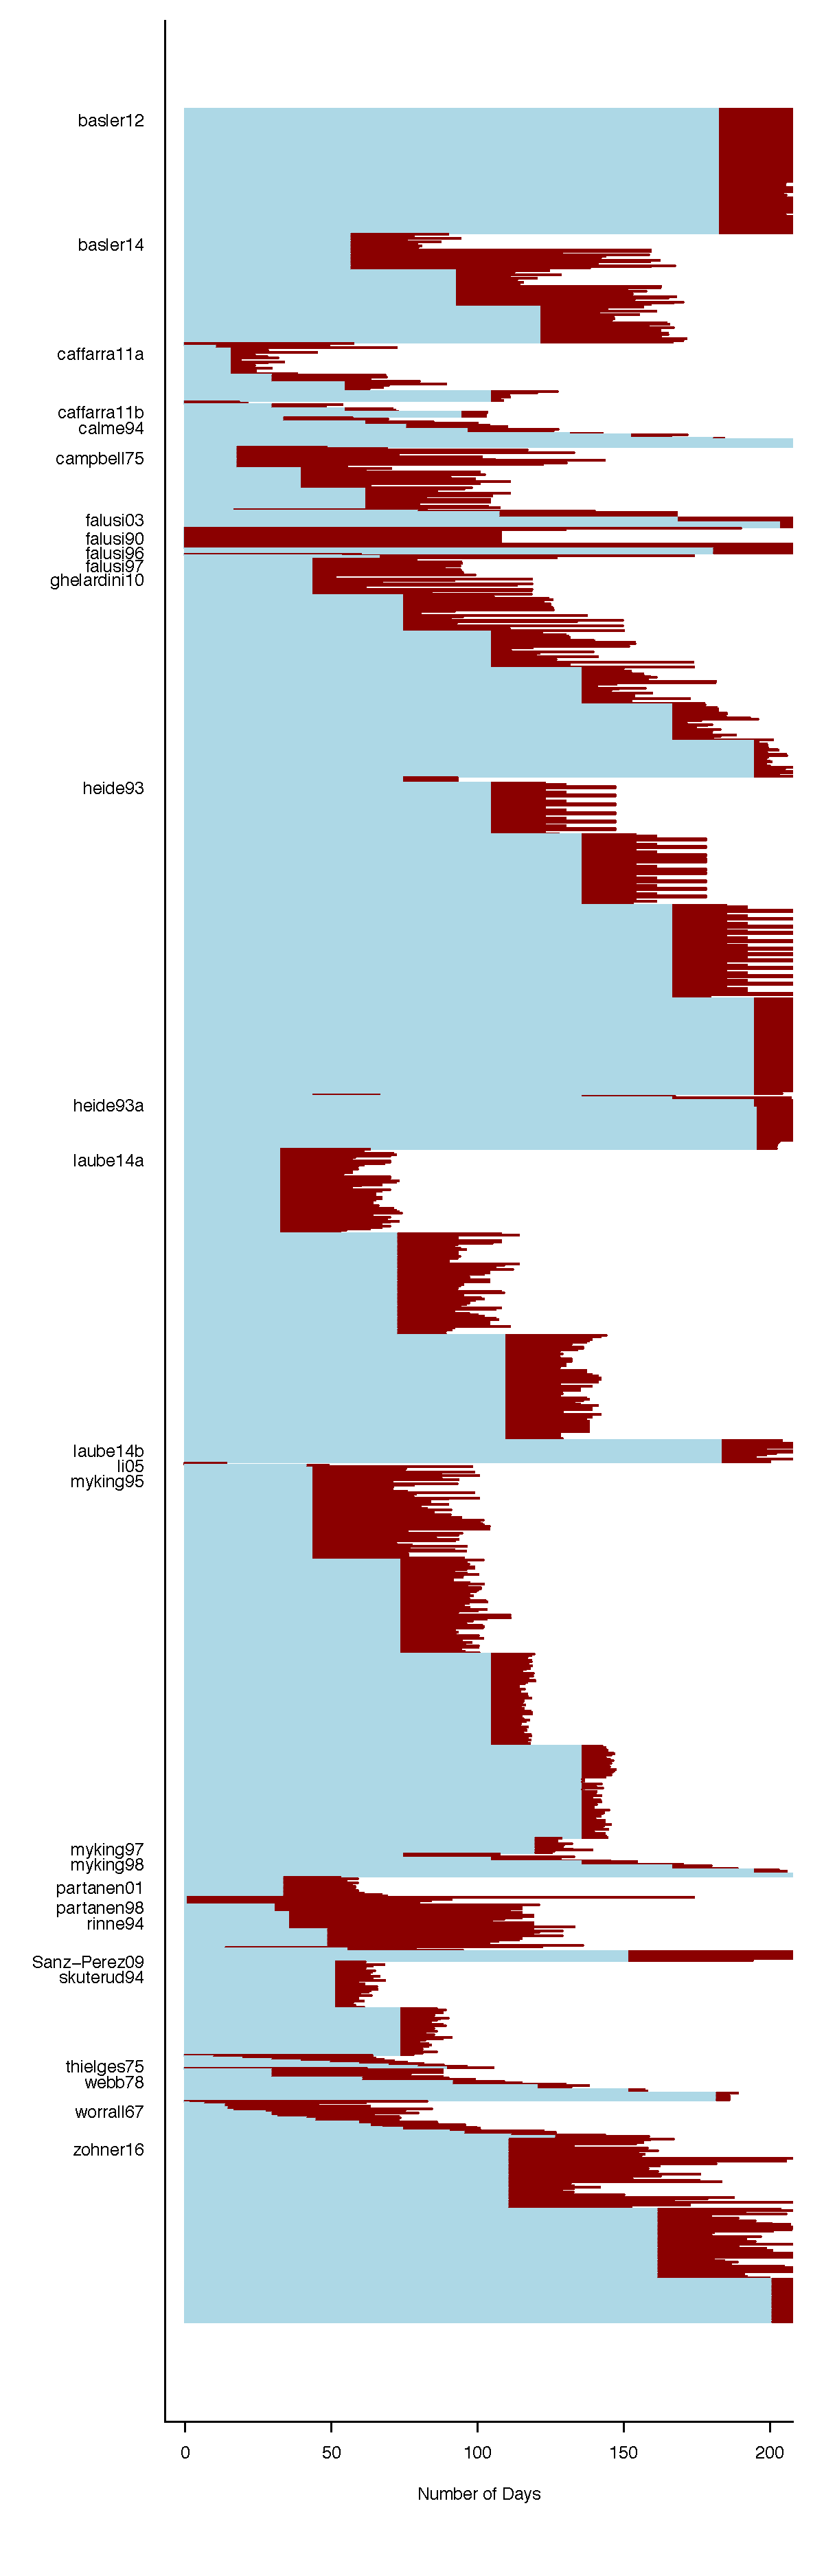
\includegraphics[width=0.40\textwidth]{..//..//analyses/bb_analysis/figures/chilldaysforcedays2.pdf}
\caption{\textbf{Days over which chilling and forcing were accumulated}, across all data included in our main model (i.e., this represents 39 studies found in 28 papers studies). Paper name is on the x-axis; blue bars represent chilling treatment length; red bars represent forcing length (i.e., days to budburst, after chilling treatments ended).}
\label{fig:chillforceplot}
\end{figure}
 \newpage


 \begin{figure}[h!]
 \centering
 \noindent 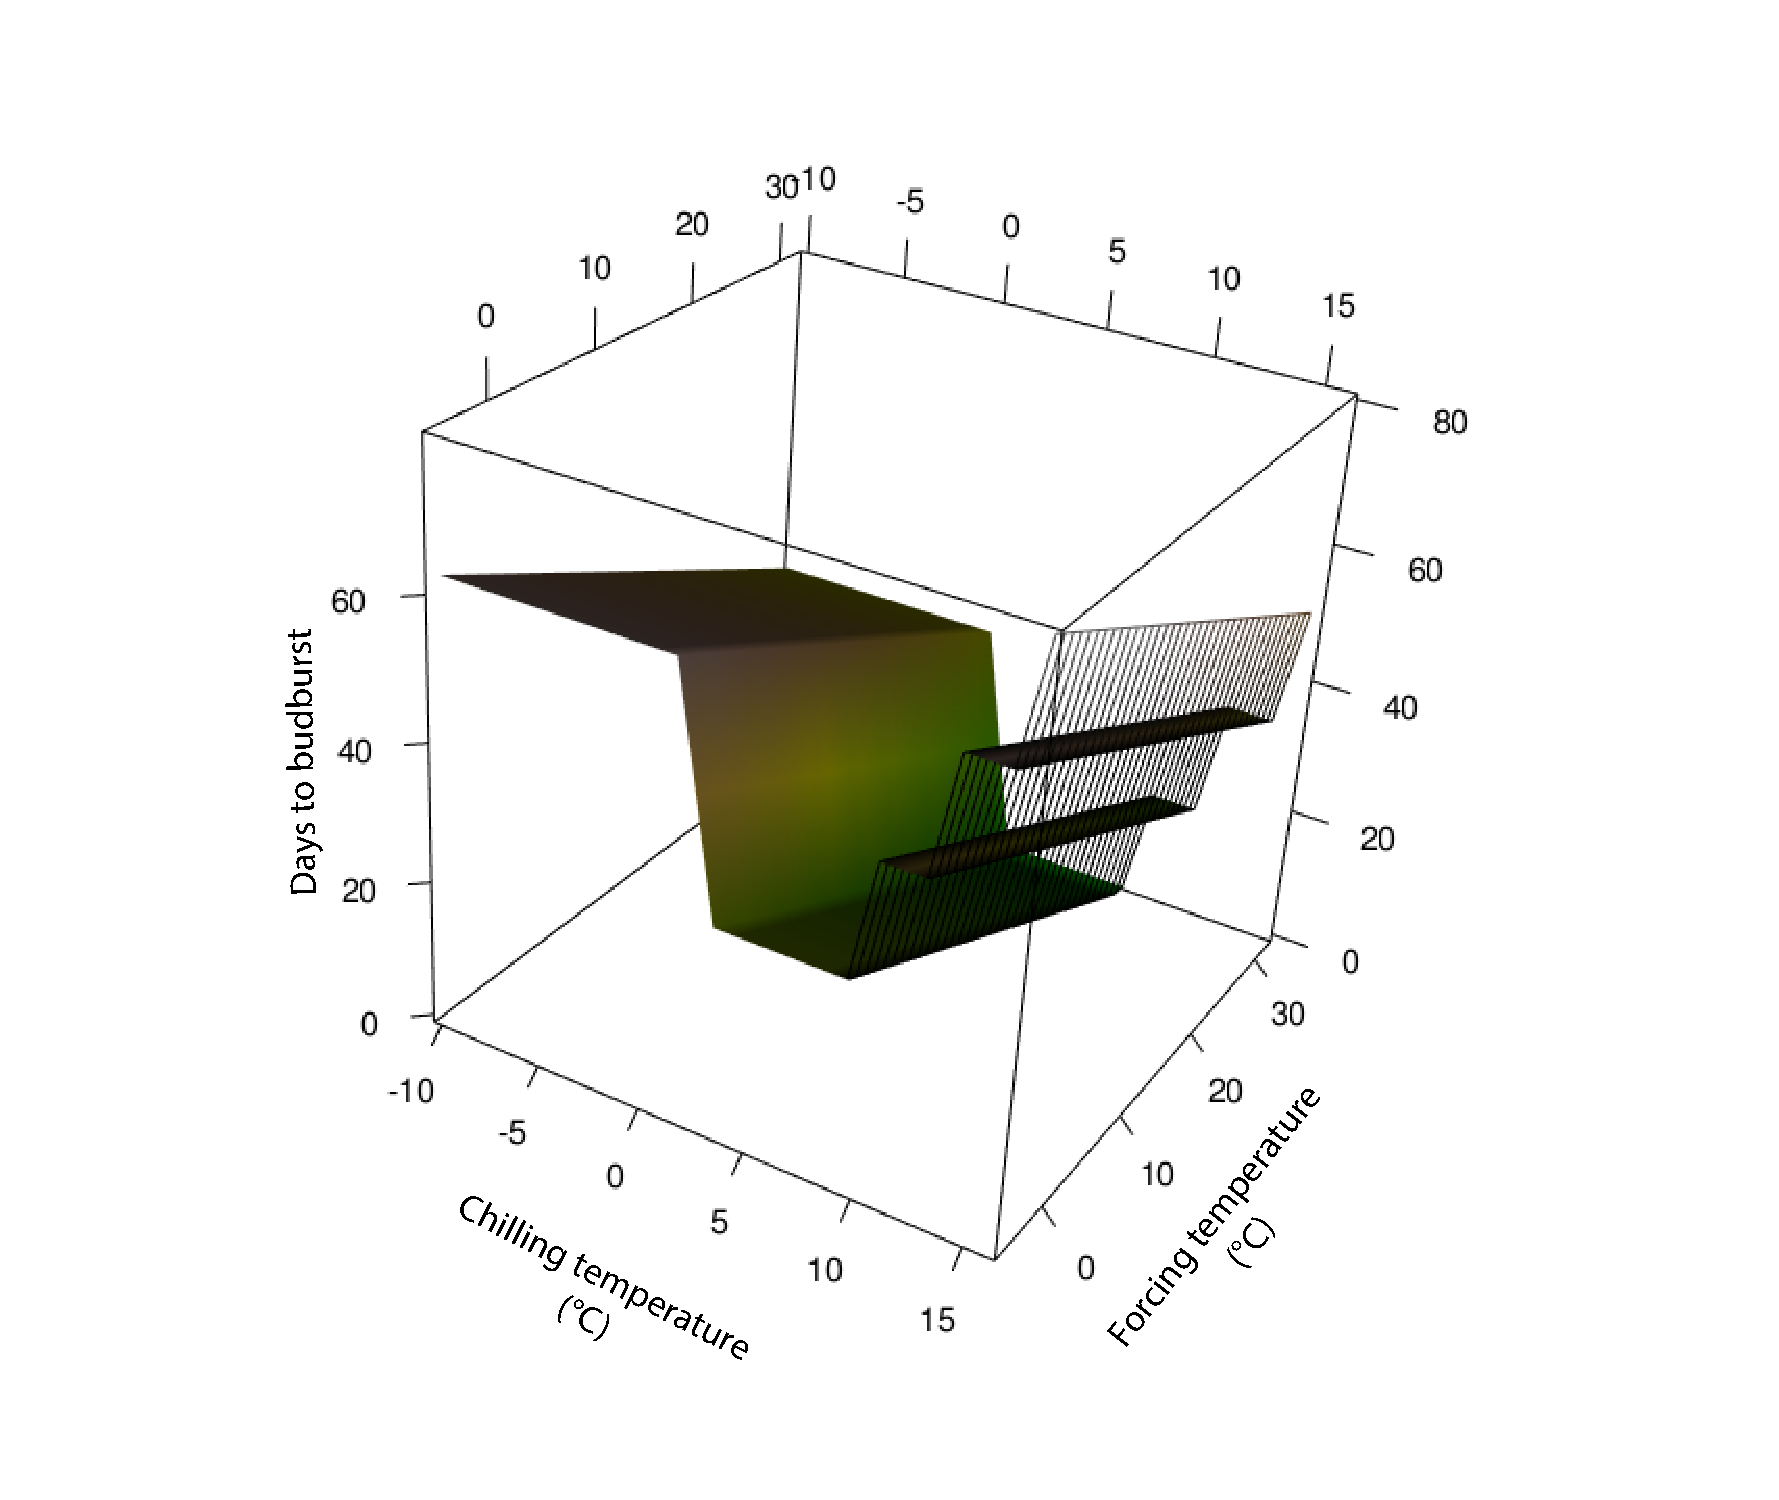
\includegraphics[width=0.75\textwidth]{..//..//analyses/bb_analysis/figures/bbmod_3dplot_utah.pdf}
 \caption{\textbf{Estimates of budburst across a range of forcing temperatures and estimated chilling} (converted to a representative mean temperature, see \emph{Estimating chilling} in the Supplemental Materials) based on overall estimates of chilling and forcing effects (Fig. \ref{fig:mu}). Maximum advances in budburst occur at intermediate chilling temperatures (\emph{e.g.}, here at mean winter temperatures of 6-7\degree C) and the highest forcing (here at 32\degree C). We set photoperiod to eight hours, which is the most common photoperiod treatment in the database. Note that days to budburst is relative to experimental methods and thus is not comparable to day of year in the field; shading represents days to budburst. Compare this to Fig. \ref{fig:3dfieldchillutah} in the main text, which uses climate data and relationships from field chilling conditions to convert chill temperature to total chilling; this figure uses the experimental treatment conditions to estimate total chilling (see `Estimating chilling' in \emph{Methods} and Fig. \ref{fig:chillexpfield} for details).} 
 \label{fig:3dexpchillutah}
 \end{figure}
 \newpage

\begin{figure}[h!]
\centering
\noindent 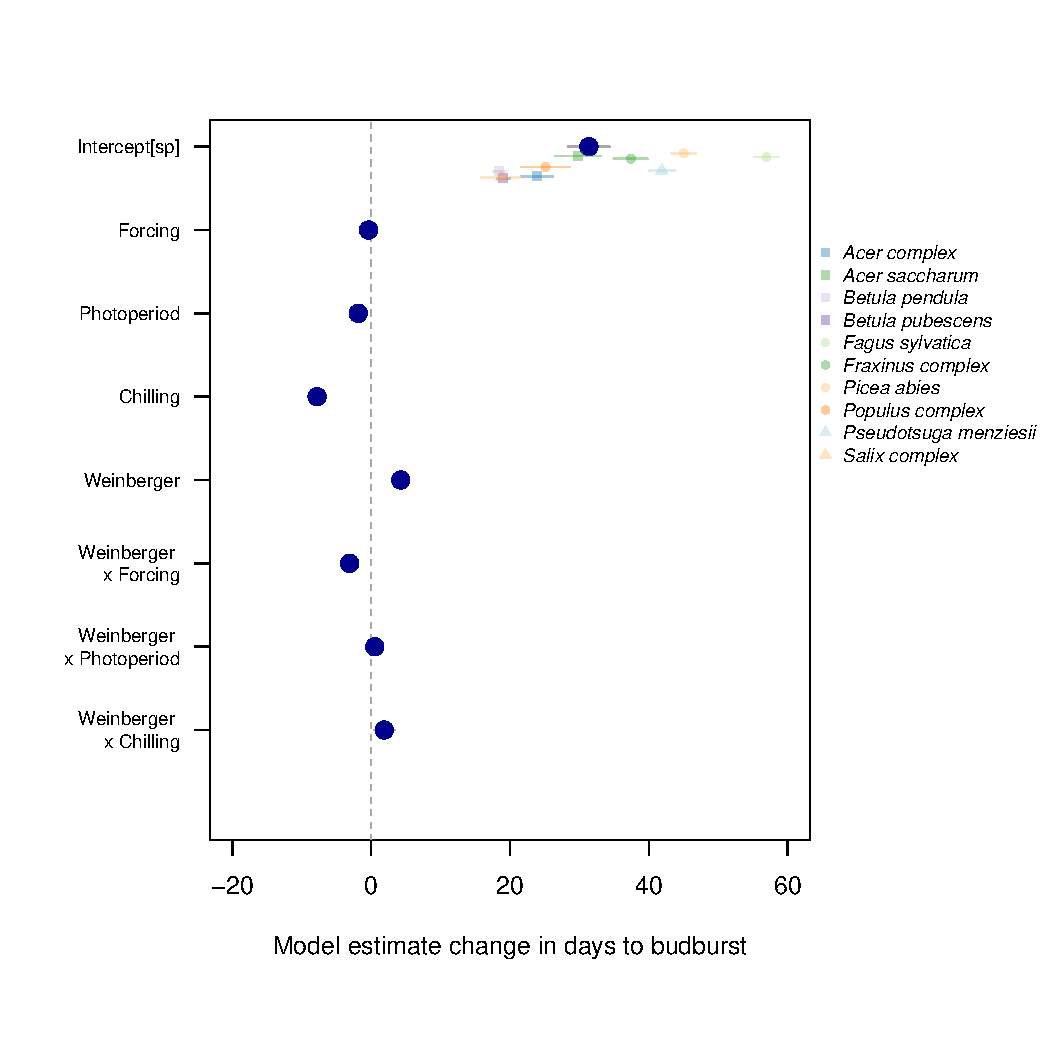
\includegraphics[width=0.75\textwidth]{..//..//analyses/figures/weinberger_MU_4supp.pdf}
\caption{\textbf{Chilling study design affects estimates of major cues.} Studies using the ``Weinberger'' method (sequential removal of tissue from field) had later budburst timing, stronger estimates of forcing (Weinberger x Forcing) and weaker estimates of chilling (Weinberger x Chilling) compared to studies that experimentally manipulated chilling directly. For an extended description of model and underlying data see \emph{Chilling study design model}; for model summary see Table \ref{tab:methods}.}
\label{fig:weinberger}
\end{figure}

\begin{figure}[h!]
\centering
\noindent 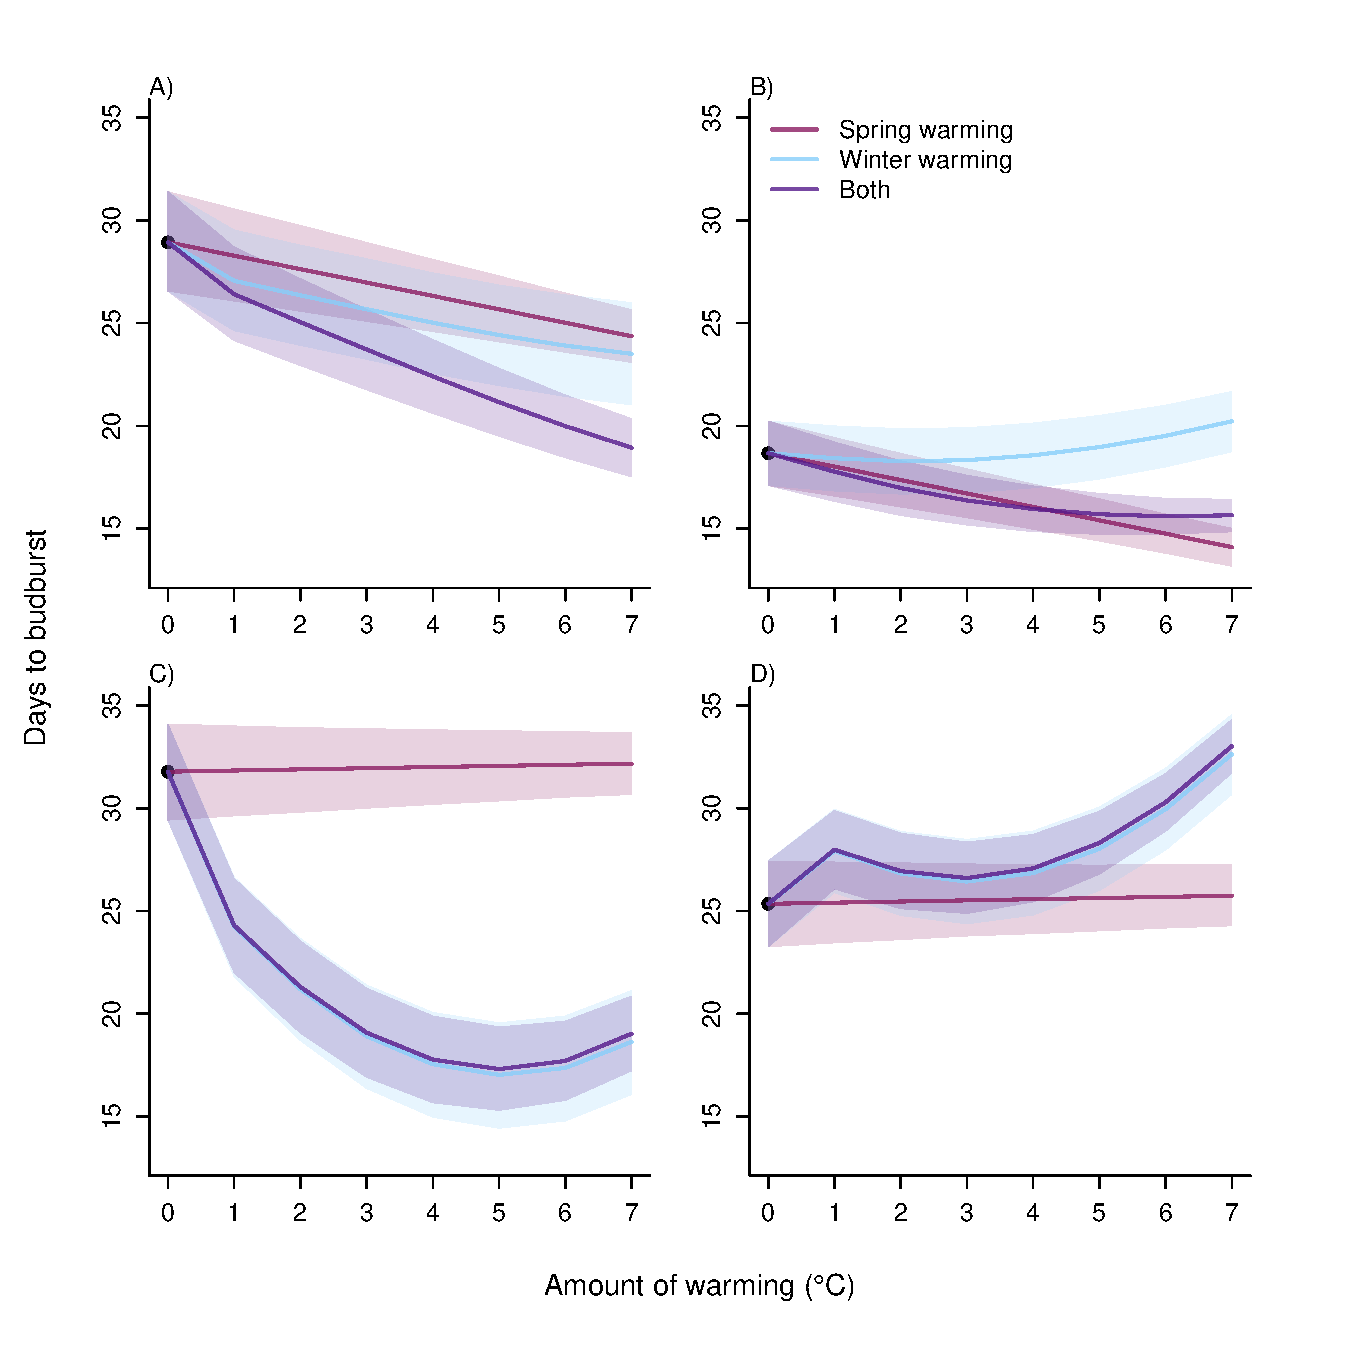
\includegraphics[width=0.75\textwidth]{..//..//analyses/bb_analysis/figures/forecasting/tempforecastbothspp_1_7_degwarm.pdf}
\caption{\textbf{Implications of warming on budburst timing varies across species and sites}, depending strongly on pre-warming climate conditions related to chilling for each site. Here we show species-level estimates from our model (Fig. \ref{fig:mu}) for the two most common species in the OSPREE database: \emph{Betula pendula} (A, B) and \emph{Fagus sylvatica} (C, D), for sites that highlight the diversity of possible budburst responses to warming (Fig. \ref{fig:foremap}, which shows general trends across many sites in Central Europe). In some sites, warming increases total chilling estimates (A, C) leading to greater advances in budburst (compared to forcing alone), whereas warming decreases total chilling estimates in other sites (B, D), leading to smaller advances and, eventually, delays with substantial warming. Compare this Fig. \ref{fig:betfag3d} in the main text, which shows all possible combinations of winter and spring warming in a three-dimensional plot.}
\label{fig:betfag2d}
\end{figure}

\begin{figure}[h!]
\centering
\noindent 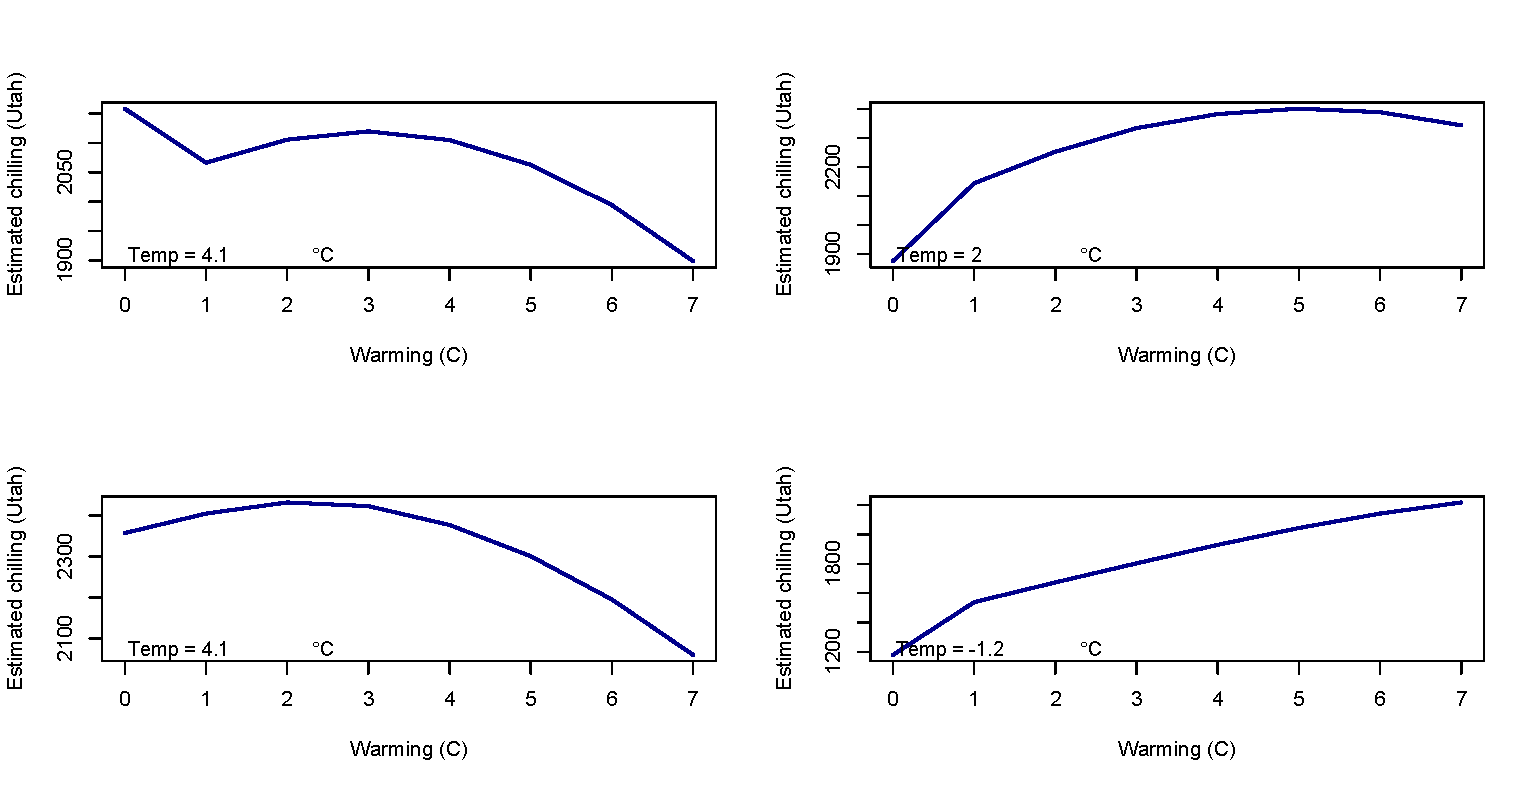
\includegraphics[width=0.75\textwidth]{..//..//analyses/bb_analysis/figures/forecasting/chillforecast_bothspp_PEP_utah.pdf}
\caption{\textbf{Implications of global warming on chilling vary by site}, depending on pre-warming climate. For sites in A (lat, lon) and D (lat, lon), chilling increases with warming, whereas chilling decreases with warming for the sites in B (lat,lon) and C (lat,lon). Compare to Fig. \ref{fig:betfag2d} and Fig. \ref{fig:betfag3d} in the main text.}
\label{fig:chillfore}
\end{figure}

%%%%%%%%%%%%%%%%%%%%%%%%%%%%%%%%%%%%%%%%
\end{document}
%%%%%%%%%%%%%%%%%%%%%%%%%%%%%%%%%%%%%%%%
